% This is file thesis-manuscript.tex.
% It defines the template for thesis of Raffael Botschen.

% The first command in LaTeX file must be the \documentclass command.
% This command declares the type of document.
\documentclass[a4paper,11pt,twoside]{article}
% 6mm
\usepackage[width=150mm,top=25mm,bottom=25mm,bindingoffset=15mm]{geometry}
\usepackage[utf8]{inputenc}
\usepackage[british]{babel} % This command guarantees proper word hyphenation.

\usepackage[T1]{fontenc}
\usepackage[mono=false]{libertine}
\usepackage{libertinust1math} % Libertine for maths
\usepackage[table,x11names]{xcolor} % For coloured text

%\bfseries
% Here we customize (sub)(sub)section name font(s).
\usepackage{titlesec}
\titleformat{\section}
  {\sffamily\scshape\LARGE}
  {\thesection}
  {0.5em}
  {}  
\titleformat{\subsection}
  {\sffamily\Large}
  {\thesubsection}
  {0.5em}
  {}  
\titleformat{\subsubsection}
  {\sffamily\large}
  {\thesubsubsection}
  {0.5em}
  {}
\titleformat{\paragraph}
  {\sffamily\normalsize}
  {\theparagraph}
  {0.5em}
  {} 

% This prevents a too long URL from staying in the same line.
\PassOptionsToPackage{hyphens}{url}
\usepackage[plainpages=false]{hyperref} % Package to create hyperlinks. Do NOT remove its option!

\usepackage{booktabs} % Package for neat tables
\usepackage[figuresright]{rotating} % Package to rotate tables
\usepackage{siunitx}  % Package to align numbers in tables

\usepackage{graphicx} % Package to load images

\usepackage{thesisTitleZEST} % ZEST title page

%\usepackage{amsmath} % Package to typeset some serious maths
\DeclareMathOperator*{\argmax}{arg\,max}

\usepackage{amsthm} % Package to typyset mathematical theorems, definitions etc.
\theoremstyle{definition} % Theorem style with boldface title and non-italicized body.
\newtheorem{definition}{Definition} % This command defines "definition" environment.
\newtheorem{property}{Property} % This command defines "property" environment.
\newtheorem{example}{Example} % This command defines "example" environment.

\usepackage{relsize} % Package to resize text, including maths symbols, e.g., sum sign

\usepackage{subcaption} % Package to enable `subfigure' environment

\usepackage{enumitem} % Package to control the vertical space between items in the lists

% Bibliography management
\usepackage[square, authoryear]{natbib}
\bibliographystyle{abbrvnat}

% This command sets citation in paranthesis as a default.
\renewcommand{\cite}[1]{\citep{#1}}

% The next three commands are needed to altername page numbering.
\newcommand\covermatter{%
  \pagenumbering{Alph} % This command ensures Uppercase letters for page numbers in PDF-reader.
  \pagestyle{empty} % This command removes page numbering until changed otherwise.
}
%  
\newcommand\frontmatter{%
  \cleardoublepage
  \pagenumbering{roman}
  \pagestyle{plain} % This command launches page numbering back.
}
%
\newcommand\mainmatter{%
  \cleardoublepage
  \pagenumbering{arabic}}
%

% This command typesets BibTeX logo
% as pointed out by Stephan Kolassa
% on https://tex.stackexchange.com/questions/18089/
\def\BibTeX{{\rm B\kern-.05em{\sc i\kern-.025em b}\kern-.08em
    T\kern-.1667em\lower.7ex\hbox{E}\kern-.125emX}}


\setcounter{secnumdepth}{4} % This command sets the level of numbering (default for "article" is 3).
%\setcounter{tocdepth}{4} % This command set the level of numbering in the table of contents.


% Formatting for code examples.
\usepackage{listings}
\usepackage{color}

\definecolor{dkgreen}{rgb}{0,0.6,0}
\definecolor{gray}{rgb}{0.5,0.5,0.5}
\definecolor{mauve}{rgb}{0.58,0,0.82}

\lstset{frame=tb,
  language=Python,
  aboveskip=3mm,
  belowskip=3mm,
  showstringspaces=false,
  columns=flexible,
  basicstyle={\small\ttfamily},
  numbers=none,
  numberstyle=\tiny\color{gray},
  keywordstyle=\color{blue},
  commentstyle=\color{dkgreen},
  stringstyle=\color{mauve},
  breaklines=true,
  breakatwhitespace=true,
  tabsize=3
}


% Table formatting.
\usepackage{array}

% Used to style thesis statement.
\usepackage{csquotes}

% Used to include pdfs for appendices.
\usepackage{pdfpages}

% Used to add captions to appendix elements that should not show up in table of figures.
\usepackage{caption}



% End of the preamble, start of the document body.
\begin{document}

%% This command ensures that the columns of type S, i.e., comma-aligned by "siunitx"
%% do not take extra space.
%\setlength\tabcolsep{3pt} 

% This command removes page numbers on the title (cover) pages.
\covermatter

%%%%%%%%%% PLEASE FILL IN YOUR INFORMATION PROPERLY %%%%%%%%%%
\author{Raffael Botschen}
\email{raffael.botschen@uzh.ch}
\legiNo{17-935-867}

\thesis{Bachelor's Thesis}
% Please double-check the correct capitalization 
% of the title on https://capitalizemytitle.com/
\title{Improving CodeDiffVis for Code Review Visualizations}

\supervisor{Prof. Dr. Alberto Bacchelli\\Enrico Fregnan}
\researchGroup{Zurich Empirical Software Engineering Team}
%%%%%%%%%%%%%%%%%%%%%%%%%%%%%%%%%%%%%%%%%%%%%%%%%%%%%%%%%%%%%%

% This command creates a bookmark in the .pdf for the title page.
\pdfbookmark[1]{Title Page}{Cover}

% This command builds the title page.
\maketitle

% This command keeps page numbering in roman style.
\frontmatter


\phantomsection
\addcontentsline{toc}{section}{Abstract} % This command includes this section from
\section*{Abstract}
Code review is an important part of modern software development and is commonly done change-based. For this, understanding the code change is a key factor for it to be effective, and tool support is needed. CodeDiffVis is a prior tool for Java that aims to support reviewers by visualizing the call and dependency graph between code entities in a code change. Due to the positive reception, we decided to improve it. We add support for Python and functional programming, as well as multi-language code changes. We evaluate our tool in a series of interviews and an online questionnaire. Reviewers responded positively, thinking it is useful for gaining an overview.
\newpage

\phantomsection
\addcontentsline{toc}{section}{Zusammenfassung} % This command includes this section from frontmatter to the Table of Contents.
\section*{Zusammenfassung}
Code review ist ein wichtiger Teil moderner Softwareentwicklung und wird häufig änderungsbasiert durchgeführt. Dafür ist Verständnis ein Schlüsselfaktor, und Unterstützung durch Werkzeuge ist nötig. CodeDiffVis is ein existierendes Werkzeug für Java das Reviewer unterstützen will indem es den Funktionsaufruf- und Abhängigkeitsgraph zwischen Entitäten im Code visualisiert. Aufgrund der positiven Rückmeldungen haben wir entschieden es zu verbessern. Wir implementieren Unterstützung sowohl für Python und funktionales Programmieren, als auch für Änderungen in mehreren Sprachen. Wir evaluieren unser Werkzeug in mehreren Interviews und einem online Fragebogen. Reviewers gaben positive Rückmeldungen, und dachten es sei nützlich um einen Überblick zu bekommen.
\newpage



% This command adds the table of contents
\currentpdfbookmark{\contentsname}{toc}
\tableofcontents
\newpage
\listoftables
\listoffigures
\newpage 
% Uncomment this if your text finished on the odd page.
%\thispagestyle{empty}
\cleardoublepage

% This command keeps page numbering in arabic style.
\mainmatter


\section{Introduction} \label{Sec:Introduction}

When the concept of code review was first described by Fagan in 1976, it was a strict and formal process based on code inspection \cite{Fagan-1976}. Since then, the usage in software projects has evolved to be more flexible and lightweight, with a multitude of tools being developed to support code reviews \cite{Rigby-2012}. The modern approach called Modern Code Review is mostly change-based and supported by tools, with changes being generally reviewed by only one or two reviewers in an informal and asynchronous process \cite{baum2016need}. In addition to these changes in process, the benefits and goals of code reviews have also changed. Identifying defects is still perceived as the primary goal, with benefits observed in practice being knowledge transfer, team awareness and the creation of alternate solutions \cite{6606617}.

Code reviews have been widely adopted in industry \citep{rigby2013convergent, baum2016need}, but there remain challenges when doing code review. Especially large changes are a significant challenge in code review, with keeping track of the review progress becoming increasingly difficult \citep{baum2016need, Baum2019}. Apart from size, Kononenko et al. have also linked higher change complexity to an increased difficulty of performing a review, because a reviewer needs to understand the code change in its greater context \cite{kononenko2016code}. 

Overall, a key finding is that understanding the review artifact is the most important aspect of reviewing code \citep{baum2016need, McIntosh-2016}. Similarly, Bacchelli and Bird have also found that understanding context and change is the key factor in a review \cite{6606617}. Another factor are the limited cognitive resources of developers, which negatively impact code review effectiveness for larger changes \cite{Baum2019}. Tools could in theory help improve understanding and reduce mental load, and in practice there has indeed been a wide adoption of tools supporting the code review process. But there still is potential for further improvements in these tools to increase review efficiency and effectiveness \cite{baum2016need}. 

Based on these findings, various solutions that could improve the code review process have been researched. One approach is to improve review efficiency by improving code understanding using automated tools for static analysis. They can be run before the review to make the results available at review time. An example for such a tool is SonarQube\footnote{https://www.sonarqube.org/}, which can be used from within the programmers integrated development environment (IDE). Another area of improvement is the ordering of code changes in change-based code reviews \cite{baum2016need}. By grouping together related changes, a graph can be constructed to guide a reviewer through a code review \cite{baum2017optimal}. And to ensure that the reviewer understands the changes, developers with experience in the frameworks and concepts used can be selected, for which a solution based on mining the potential reviewers' project comments has been proposed \cite{DBLP:journals/corr/abs-1906-07108}. 

Tools like GitHub\footnote{https://github.com/} and the open-source equivalent GitLab\footnote{https://gitlab.com/} present the code changes and their contexts, to make it easier to see which code was deleted, added or changed. But they don’t offer support for developers for understanding the code changes. This can be inefficient, especially with larger and or more complex code changes. 

The paper by Fröhlich has shown that providing a visual overview of the code changes is beneficial \cite{publication-20661}. They developed a tool called CodeDiffVis (or ReviewVis) to analyze Java source code to construct a combined dependency and call graph, which would then be displayed when doing code review. The aim was to make the information flow within the change faster and easier to understand. When evaluated, they found that for improving developers’ understanding, their tool was generally perceived positively when it comes to usefulness. In a follow-up study, these findings were confirmed \cite{cr_visualization_major}.

One of the main limitations identified by Fröhlich was the lack of support for multiple programming languages, which limited the usefulness of ReviewVis \cite{publication-20661}. To address this, we extended the language support to include Python. This entailed extending the concept of graph visualizations to functional programming. We also implemented support for automatically handling graphs containing multiple programming languages.

We evaluated our implementation in a series of interviews with developers. When possible, collected feedback was used to iteratively improve the tool. Further information was collected in an online questionnaire for the interviewees. Participants responded positively to the tool, finding it easy to learn and useful to gain an overview over a changeset. They would like support for more programming languages and means of integrating ReviewVis with other tools.

\newpage


\section{Problem Description} \label{Sec:ProblemDescription}
In this section we explain the tool we expanded and improved in more detail, shortly describing the technical implementation and developers feedback. Then we present the goal of this thesis and how we achieved it.

\subsection{Visualizations and ReviewVis}  \label{SubSec:VisualizationsAndReviewVis}
One approach to improve the critical understanding of the code under review is enhanced tool support for the reviewers. This could be done with visualizations, and in a study done by Fröhlich they indeed found that most developers who participated in their study thought visualization tools could benefit code review \cite{publication-20661}. Despite this, only a minority used any. This seems to indicate an opportunity to improve the code review process. 

Fröhlich developed the tool ReviewVis (previously CodeDiffVis) to create such visualizations \cite{publication-20661}. Their tool consists of two parts: CodeDiffParser (CDP) analyzes Java source code to create a call and dependency graph. Taking advantage of the findings of Baum and Schneider that code reviews are commonly done change based, their tool analyzes code changes to only extract the information relevant for the review. This can be exported to a file. An extension for Google Chrome called CodeDiffVis (CDV) then loads the information from this file to draw the graph for merge requests. This graph is customizable and interactive, and can be displayed alongside the code change under review. 

When evaluating this tool, they found that most participants would like to use the tool, and that it provides useful information. Of interest is also that it was well received for large code changes of 8 or more files, which was the area identified by Baum and Schneider as the most significant challenge. Not all parts of the tool were received as well, with less positive feedback for graph customization features and lack of support for keeping track of a review. But the underlying concept was received well, which in our opinion made further work on it justified.


\subsection{Motivating Example} \label{MotivatingExample}
To understand a changeset, the reviewer needs to either be already familiar with the project, or should be able to understand it easily. When doing the review, the reviewer then needs to keep the structure and context of the code in their mind. This means extracting the code entities like classes, methods and functions and analyze how they depend on each other. Furthermore they need to understand the call flow between these entities to understand how they interact. To do this, the code needs to be navigated and searched to find these entities and relations between them. Our tool addresses this problem by extracting this information and visualizing it in a graph, to reduce the cognitive load on developers.


\subsection{Goal of this Thesis} \label{SubSec:DescGoal}
One of the main limitations of Fröhlich's tool was that the backend consisting of CDP only supported Java code. The frontend (CDV) was language agnostic in theory, but supported only an object-oriented programming style and included features primarily useful for Java code. This limited its usefulness to only this language and meant that it could only be evaluated for Java code.
\\

The thesis statement is as follows:

\begin{displayquote}\textit{ReviewVis is a useful tool for code review visualizations for both Python alone and Java and Python together.}
\end{displayquote}

To enable us to validate our thesis, we implemented a Python version of CDP to analyze Python code. For this, we introduces a number of new code entities to represent different code. The frontend was extended to support functional programming and other features. Parts of it were also rewritten to automatically handle arbitrary combinations of languages. This allows ReviewVis to support Python code, and graphs with multiple languages.

We evaluated ReviewVis in a series of remote interviews with software developers. In them we asked developers about their perception of ReviewVis in three examples we chose: a smaller changeset, a larger and more complex changeset, and the largest changeset combining Java and Python.
Topics we focused on are the graph visualizations, means of interacting with the graph, multi-language graphs, and what their overall perception is. Developers were also encouraged to mention any other feedback they had.
Furthermore, they answered an online questionnaire using the Technology Acceptance Model to quantitatively assess their perception of the tool and future adoption.
We validate out hypothesis by analyzing the interview recordings and answers from the online questionnaire.

\newpage


\section{Related Work} \label{Sec:RelWork}

\subsection{Source Code Visualization} \label{SubSec:SCVis}

Modern integrated development environments (IDEs) like Visual Studio Code and PyCharm typically present source code divided by files. Depending on the programming language and paradigm, in most cases each file contains one or more code entities. These can be classes in the case of object-oriented programming (OOP) or functions in case of functional programming (FP). Focusing on the file-structure has the advantage that it is nearly universal between languages and operating systems, making it easier for single IDEs to support many languages, while users of them can use a common interface. 

But in only considering the file structure, the often more important logical structure of the code (i.e., the software entities and their relations) is not considered, which can introduce some problems. One is that because all file contents including whitespace are displayed, display space is wasted. Another one is that frequently code that is irrelevant to the user is displayed, with the relevant code fragments being at a different position within the file or another file altogether. This makes frequent navigation in the code necessary for users to get all relevant information. These problems have been recognized, and many researchers have searched for possible solutions \cite{10.1145/1165734.1165736, bragdon2010code, Deline2012}.

One approach is the bubble metaphor, introduced by Bragdon et al. \cite{Bragdon_2010}. A bubble is an editable code fragment. Multiple bubbles can be displayed concurrently, to show all and only the relevant code fragments instead of single whole files. In theory this reduces time needed for navigating code, and indeed Bragdon et al. found in another study that, in a quantitative experiment, their Code Bubbles IDE significantly reduced both the time required for navigation and understanding code \cite{bragdon2010code}. 

Another approach, which was used in this thesis, is the representation of source code using graphs. Nodes can represent whole files or code changes, or features of the code like classes and methods, or functions in OOP and FP respectively. The edges represent the relations between the nodes, and can be call based or dependency based. Call based relations, i.e. method or function calls from node A to node B, with both nodes being classes or functions, result in a call graph. Dependency based relations, where the relations represent dependencies between features (e.g., object creation of one class in another), result in a dependency graph. Such a graph can also be created for only parts of the whole codebase, i.e. a code change in the context of a code review. Baum et al. introduced the approach of constructing a graph based on the relatedness of code changes (as measured by a multitude of factors) in 2017 as the result of searching for an optimal ordering of change parts \cite{baum2017optimal}. Our approach is explained in more details in chapter \ref{Sec:DesignImplementation}.


\subsection{Code Collaboration, Version Control Using Git and Code Review}  \label{SubSec:CodeCol+VersCntrlGit+CodeRev}

Since its introduction by Fagan in 1976 \cite{Fagan-1976}, code review has become an important part of the software development process. While the original code inspections as first proposed by Fagan were very time and resource consuming, the modern code review process has shifted from a formal and structured process to a more informal one \cite{6606617}. Bacchelli and Bird introduced the term Modern Code Review (MCR) to describe the change-based, lightweight, and tool-supported approaches that are commonly seen practiced today \cite{6606617}. MCR is performed in a peer review style, where the changes are reviewed by one or more developers (the approvers), which are different from the developer who wrote the code change (the author). Reviewers can give feedback in comments or approve the code change. Bacchelli and Bird identified many advantages of code review, with improved knowledge transfer and the creation of alternate solutions among them. At the same time, the detection of defects, while commonly seen as one of the main reasons for doing code review, was limited in practice \cite{6606617}. 

A popular tool for versioning is Git\footnote{https://www.git-scm.com/}. When using Git, a set of changes to the code are combined into a commit, which represents a new version of the code base. Multiple concurrently active code bases are supported by splitting them into branches. This way there can be a release branch which is the main code base, branches for untested beta software, and branches that contain work in progress like new features. When work on a branch is finished, e.g. when a feature is complete, the branch can be merged into another one, meaning the branches are united. This can be done in multiple ways. When merging two branches the source code bases are simply compared, whereas rebasing tries to preserve the individual commits made to the branches in their temporally correct order. This has implications for tools which analyze the ordering of commits. 

The importance and popularity of code review in modern times has led to the creation of many tools to support code review, with well-established code reviews being based on Git. These include GitHub\footnote{https://www.github.com/}, which is owned by Microsoft, and the open-source alternative GitLab\footnote{https://www.gitlab.com/}. They have source code versioning management capabilities and can support code review. This is done by showing changes from commits or merge requests in their web interfaces based on a git diff view, showing the added and deleted source code parts. In code review the reviewer can then use this for their review. This change-based review process is commonly done today \cite{6606617}. 

Other web-based tools supporting versioning management and code review support include Phabricator\footnote{https://www.phacility.com/phabricator/} and Gerrit\footnote{https://www.gerritcodereview.com/}. Phabricator is an open-source project originating from Facebook which supports multiple version control systems like Git, SVC and Mercurial. It also supports issue tracking which Gerrit lacks. Gerrit is an open-source project initially developed by Google. Its strength is code review support and tracking commit changes.

\subsection{Related Tools and Concepts} \label{SubSec:RelTools+Conc}

\subsubsection{Approaches to Improve Reviewers’ Understanding of Code} \label{SubSubSec:ImprovCodeUnderstanding}
Change Part Ordering is an approach proposed by Baum et al. to facilitate code review \cite{baum2017optimal}. Tools like Gitlab currently display code changes in alphabetical order. Baum et al. proposed that changing the order in which these code changes are displayed could reduce cognitive load and found that an optimal order is grouping together related changes \cite{baum2017optimal}. Relatedness is determined using the underlying call graph of the code change. But this does not account for other possible relations that are not helped with this approach, like when changes are in the same file. Therefore we believe that although employing this theory would reduce the navigation within the code change and thereby reduce reviewers’ cognitive load, it could be reduced more significantly by file-independent visual support focusing more directly on the relatedness. 

Another approach, tackling the automatic decomposition of changesets for code review, is the tool ClusterChanges by Barnett et al. \cite{7194568}. They observed that despite best practices recommending otherwise, changesets often contain multiple independent changes. This complicates the code review process, because developers need to mentally decompose the changes. To address this, their tool partitions the code changes into different partitions, and shows them in a tree view. By selecting a specific partition, all related changes can be listed. It was meant to validate the proposed use case. They found that, evaluated on C\# code within their organization, ClusterChanges can indeed decompose such changesets in a way that developers agree with the proposed decomposition. A replication study by Luna Freire et al. replicated this finding for open-source Java projects \cite{10.1007/978-3-319-73117-9_18}.

\subsubsection{Tools to Assist in Code Review } \label{SubSubSec:CodeRevTools}
Softagram analyzes source code and its dependencies of merge requests. It supports a wide range of code versioning platforms including Gitlab, GitHub, Bitbucket, Azure and Gerrit, as well as various programming languages (including Java, Python and C++). A merge request triggers an analysis, the result of which is posted as a graph in the comments. This graph includes added and removed dependencies, as well as hidden or unwanted dependencies. Dependencies can also be shown on per-package or per-class level. Softagram focuses on dependencies, with rules helping with the detection of erroneous dependencies. This focus on dependencies only means that call graphs cannot be produced, meaning there is only partial overlap between it and ReviewVis. 

Ho-Quang et al. developed a tool similar to Softagram for whole project inspection called RoleViz \cite{ho2019towards}. They make use of the notion of role-stereotypes introduced by Wirfs-Brock in 2006, which categorizes the type of functionality that a class has within a system, as well as typical types of interaction with other classes \cite{1605171}. RoleViz uses the most common role found in a class as this class’ main role. Packages are analyzed similarly with respect to dependencies between each other. Based on this a visualization is created. In a study by the same author they compared it to Softagram using a complex Java project, and found that it has better results for comprehension tasks, while not increasing the cognitive load \cite{truong2019empowering}. Participants identified the need for behavioral information like call graphs as a limitation of the tool \cite{ho2019towards}.

\newpage


\section{Background} \label{Sec:Background}
To create an abstract representation of source code like a graph, the code first must be parsed to create a hierarchical representation. From this the elements that are of interest can be collected: e.g., classes, methods, functions, etc. Connections between these elements like dependencies and method or function calls can be collected or inferred as well. This chapter explains how this can be done for Python source code. In chapter \ref{SubSec:AST} we first talk about Abstract Syntax Trees (ASTs) as a possible abstract source code representation. Chapter \ref{SubSec:ModulesSymbolsPython} talks about the challenges an limitations of Python. Chapter \ref{SubSec:CouplingDependencies} presents the dependencies that can be extracted.


\subsection{Abstract Syntax Trees (AST)} \label{SubSec:AST}

To represent parsed source code, Abstract Syntax Trees (ASTs), which are sometimes just called syntax trees, can be used. They are a hierarchical representation of source code with only the parts relevant for further analysis included, as opposed to parse trees which contain all parts of the source code \cite{cooper-2011}. This could be things like brackets, colons or comments, which may not be relevant when the AST is used, e.g. for a compiler. Python’s standard library has a module called \textit{ast}. It is used internally to create the AST of Python code, which can then be compiled into a Python code object. Using this module, ASTs can be created programmatically. Because the \textit{ast} module is used by Python itself when executing code, it is guaranteed to be up-to-date and a correct representation of the code's behavior (for the installed version). It does not resolve any names (symbols), meaning that this has to be done in a separate processing step.

Consider Figure \ref{figure:exPyProg} with some simple Python code, defining a function and a class, and using them. The AST for it which is generated using the \textit{ast} module is schematically drawn in Figure \ref{fig:PythonAST}. The AST will usually be comparatively big. The \textit{ast} module does not resolve any symbols, meaning it does not resolve class, method or function dependencies. This is different from other languages like Java, where the AST will already include some of this information. The reason is Python’s dynamic typing system, which only resolves the type at runtime.

\begin{figure}[h]
    \begin{lstlisting}
# example.py

# function definition
def bar(text):
    print(text)

# class definition
class Thing:
    # constructor
    def __init__(self, mass):
        self.weight= mass

# function call
bar("Hello") 

# variable declaration and object instantiation
obj = Thing(5)
    \end{lstlisting}
    \caption{Example Python Program containing a function and class definition. Later in the same program the function is called with a string, and a newly created object is assigned to a variable.}
    \label{figure:exPyProg}
\end{figure}

\begin{figure}[h!]
    \centering
    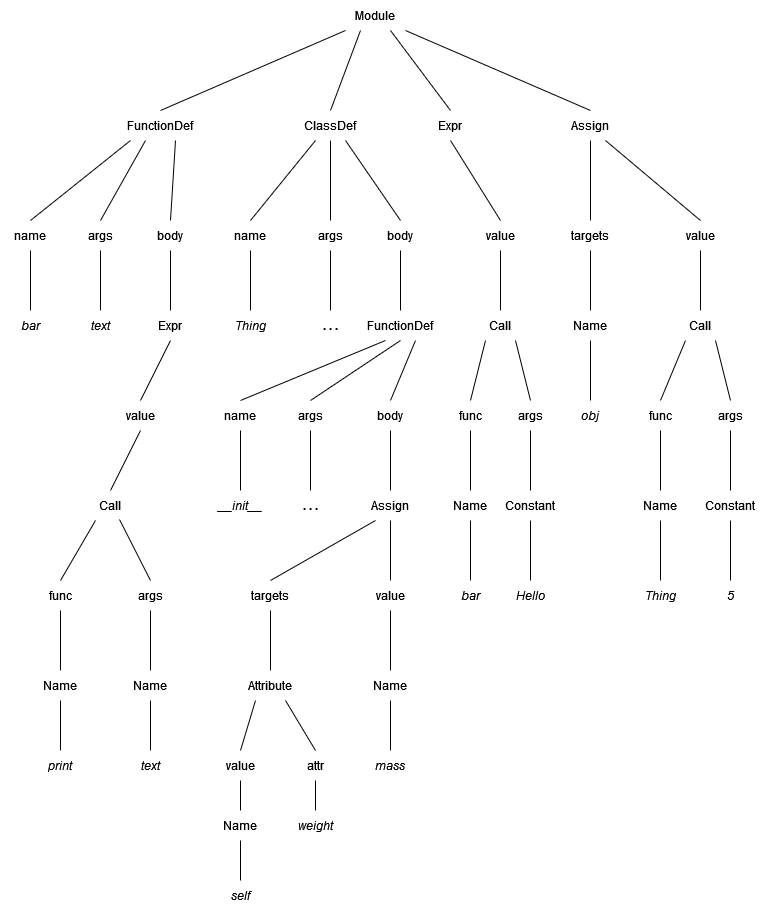
\includegraphics[width=1.0\textwidth]{Subfigures/Python_AST.png}
    \caption{Visualization of a simplified AST for the code in Listing 1 using Python’s built-in \textit{ast} module. The graph is slightly simplified for clarity. Each node stands for an object, with their children representing their members. Leaves are shown in italic. If a node has more member variables than is shown, it is indicated by a “...” symbol. A \textit{Name} node can represent any symbol, including variables, objects and function names. Symbols and bindings are not resolved by the \textit{ast} module, instead this is done at runtime.}
    \label{fig:PythonAST}
\end{figure}


\subsection{Modules and Resolving Symbols in Python} \label{SubSec:ModulesSymbolsPython}
One of the main limitations of the Python \textit{ast} module lies in Python’s typing system. In statically typed languages like Java the types are already known at compile time and can therefore be represented in an AST. Python instead makes use of a dynamic typing system where the type of objects is only known at runtime. While it is still possible to infer some information about the types in a program, the information content of the AST is limited compared to statically typed languages. Python also makes use of duck typing, where an object can be used like one of a certain type if it has all methods and properties of that type. This further complicates a static analysis of the program, because it requires further processing of the AST.

For example, imagine a function that takes an object \textit{foo} as a parameter and calls the method \textit{bar()} of that object. Figure \ref{figure:exDuckTyping} shows the source code for it. When analyzing the source code, we can infer that \textit{foo} must be of a type which has a method with signature \textit{bar()}. If we also know how this function is used, i.e. that the function is called with an object of a specific type, we can infer a connection between this function and the type (class) which gets used by it. But this is solely dependent on what information is available to us from the source code. If this function is part of a library, we cannot know how it will be used. Also, because of duck typing we can only make statements about how the function is used in the analyzed code, not how it could be used in general. Overall, this means that while we can make some deductions about the code, we generally will not be able to know everything about how the code will behave at runtime or how it can be used by other code \cite{python-software-foundation-2022}.

\begin{figure}[h]
    \begin{lstlisting}
# Takes an object and calls its method bar.
def fun(foo):
    foo.bar()
    \end{lstlisting}
    \caption{Example for a method call that cannot be resolved without additional information.}
    \label{figure:exDuckTyping}
\end{figure}

To explain how the Python interpreter resolves names, an overview of the way of structuring code in Python needs to be given first. Definitions can be put into a file, from which they can be imported. Such files are called modules, and they can contain arbitrary executable code. Several modules, the standard modules, are already built in. For bigger projects packages can be used, which can contain submodules (e.g., the module name A.B names a submodule B in package A). While single modules can be imported from packages, the author of the package can also define a standard set of modules that get imported from the package. 

Resolving a symbol happens at runtime and depends on the runtime environment. If a name is defined in the same file, resolving it is trivial and can be done using simple static code analysis. If the name is imported from somewhere, the interpreter first searches for a built-in module of that name. If it does not find it, the modules in the same directory are searched. After that, the interpreter searches a list of directories including the directory containing the input script, \textit{PYTHONPATH} (a list of directory names), and an installation dependent default. Scripts can modify these directories lists. This means that resolving names statically requires searching a wide number of directories and might not be accurate. In practice, for most programs the used names are either in the same package, or in one of the standard directories. Therefore, simple static analysis can still work accurately for most programs. 

The problems of static analysis in Python are due to its nature, and therefore have existed since its conception. With Python’s popularity came interest in this, as static analysis tools are needed for example in IDEs for automatic code completion and detection of issues. Thus, much work has been done in this area, and we were able to use a popular tool called jedi\footnote{https://www.github.com/davidhalter/jedi}, which is explained in more detail in section \ref{SubSec:Backend} when explaining the CodeDiffParser backend.


\subsection{Coupling and Dependencies} \label{SubSec:CouplingDependencies}
Coupling and dependencies are key concepts especially in object-oriented programming (OOP). Coupling is a measure of dependency among software components. To understand the connections between different nodes in the AST, a coupling analysis needs to be done to understand how they are coupled.

Dependencies are a subset of couplings. If one object is used by another, we have a dependency. For example, if a class B uses class A, A is a dependency of B because B cannot work without A. If such a dependency between two classes exists, they are coupled. 

In general, coupling relations can be divided into four high-level groups \cite{FREGNAN2019159, Bavota2013692}:
\begin{enumerate}
    \item Structural coupling: The static relations between entities in the source code, like called methods and inheritance. 
    \item Dynamic coupling: Runtime calls between classes and methods. 
    \item Semantic coupling: Entities that have similar terms in in their comments and identifiers, hinting at similar responsibilities. 
    \item Logical coupling: Entities that are frequently shared together and that therefore are logically connected.
\end{enumerate}

Bavota et al. found that semantic and structural coupling are the most important types of coupling \cite{Bavota2013692}. Semantic coupling can be extracted using more advanced techniques such as Machine Learning \cite{DBLP:journals/corr/abs-1906-07108}, which are out of the scope of this thesis. The focus of this thesis is on structural coupling, which can be determined deterministically using source code. Structural coupling relations can be divided into a small set of relations that developers are already familiar with, instead of needing to introduce coupling measures and concepts new to the developers. Structural coupling can also be inferred using well-understood algorithms for each language with known limitations. More complex techniques can introduce new failure modes and require complex calculations, slowing down the tool. 

Dependencies can be static or dynamic \cite{jenkov-2014}. Like with coupling, static dependencies refer to dependencies that can be resolved using static analysis, while dynamic dependencies can only be resolved at runtime. By parsing an AST only static dependencies can be captured. 

Jenkov identifies three kinds of dependencies, shown in Table \ref{table:DependencyTypes}. He differentiates between method dependencies, going from the method of one class to the method of another, and actual class dependencies. Unless the method dependency is part of a static class, there is a class or interface dependency as well. 


\begin{table}[h!]
\begin{center}
\begin{tabular}{ m{4.5cm} | m{9cm}} 
 \hline
 \rowcolor{lightgray} Dependency Type & Explanation \\
 \hline
 Class dependency & A class or interface that has a dependency on a class. This can be a class hierarchy dependency or a class reference, i.e., an instantiated object of another class. \\
 \hline
 Interface dependency & A class or interface that has a dependency on an interface. This can be a class implementing an interface, an interface that is extending another interface or a type reference. \\
 \hline
 Method dependency & A class or interface that has a dependency on a concrete method or field of an object. \\
\end{tabular}
\end{center}
\caption{Dependency types in OOP as described by Jenkov \cite{jenkov-2014}.}
\label{table:DependencyTypes}
\end{table}

\newpage



\section{Design and Implementation} \label{Sec:DesignImplementation}

Tool support has been identified as a potential way to support reviewers by helping them understand the code changes better. They found that there is a need to better understand especially large changes, and hypothesized that a visualization of the code change could be helpful \cite{baum2016need}. The first version of ReviewVis developed by Fröhlich et al. aimed to explore this hypothesis \cite{publication-20661}. As a first prototype, they focused on developing potential visualizations for change-based code comparisons. Java was picked to be the basis for the visualizations, as it was a popular programming language. For creating the graph they used the Eclipse AST Java parser, which was the most reliable in their testing. To display it, a browser plugin for GitLab was developed, which handles the visualization separately from GitLab itself, making it less invasive and more modular. GitLab was chosen as it is open-source and commonly used in practice by developers. When evaluating their tool, developers responded positively to the visualizations. Because the existing concept seemed to work well, this thesis kept the original structure of ReviewVis while extending it from only OOP to FP, and added support for reviewing projects using multiple languages. Python was chosen as it too was a popular language, and had support for different programming paradigms.

We first describe the elements (i.e., nodes and links) of the graph which is visualized in Chapter \ref{SubSec:PyGraphStruc}. Then we describe how ReviewVis works. In short, in consists of two components: CodeDiffParser and CodeDiffVis. CodeDiffParser analyzes a code change and extracts the graph, which can be exported to a file. It is explained in Chapter \ref{SubSec:Backend}. CodeDiffVis can then load this file and visualize the graph in the browser. It is explained in Chapter \ref{SubSec:Frontend}. We also give an example for a merge request and the visualization produced by the tool in Chapter \ref{SubSubSec:ReviewVisExample}.


\subsection{Python Graph Structure} \label{SubSec:PyGraphStruc}
The graph is formed by nodes and links connecting these nodes. The nodes contain the necessary information to understand the type and position of the node, with additional meta-information to enable various features. The links establish connections between these nodes, describing their relationships. 

Nodes contain the file path, the node name, the name of the enclosing entities (e.g., class for methods), the name of the collection of entities that it is part of (packages in Java, modules in Python), the type of node (e.g., function, class, etc.), the new and old position within the file (if applicable), the status (added, changed, unchanged, or deleted), parent node id (node within which this node was defined), the id of the node itself, a flag for if the node is generated (Java specific), and the programming language. A list of the possible node types with an explanation for each of them is given in Table \ref{table:PyNodeTypes}.

\begin{table}[h!]
\begin{center}
\begin{tabular}{m{4.5cm} | m{9cm}} 
 \hline
 \rowcolor{lightgray} Node Type & Explanation \\
 \hline
 CLASS & Class definition. \\
 \hline
 METHOD & Method definition. \\
 \hline
 FUNCTION & Function definition. \\
 \hline
 METHOD\_REFERENCE & Reference to a method (e.g., method call). \\
 \hline
 FUNCTION\_REFERENCE & Reference to a function (e.g., function call). \\
 \hline
 SCRIPT & File containing some code not part of a function or class. Useful to group together references. \\
 \hline
 TOOLERROR & The tool encountered a problem (e.g., unable to resolve call). \\
 \hline
 UNKNOWNFILE  & File not in one of the supported programming languages. \\
 \hline
\end{tabular}
\end{center}
\caption{Node types extracted from Python code.}
\label{table:PyNodeTypes}
\end{table}

The links contain the source (origin) node id, the target (destination) node id, the relation type (e.g., method call, superclass, etc.), the status (added, changed, unchanged, or deleted), and the id to identify this relation. The possible link relations and explanations for them can be found in Table \ref{table:PyLinkTypes}.

\begin{table}[h!]
\begin{center}
\begin{tabular}{m{4.5cm} | m{9cm}} 
 \hline
 \rowcolor{lightgray} Link Type & Explanation \\
 \hline
 SUPERCLASS & Links from a subclass to the superclass from which the subclass inherits. \\
 \hline
 ENCLOSING\_CLASS & Class defined within another class. Links from the inner class to the outer class. \\ 
 \hline
 METHOD & Link connecting a class to one of its methods. \\
 \hline
 METHOD\_CALL & Link connecting the node where the method call originates to the called method. \\
 \hline
 FUNCTION & Links from a (non-class) node in which the function node is contained to the function node. \\
 \hline
 FUNCTION\_CALL & Links from a node calling a function to the called function. \\
 \hline
 TOOLERROR & Links from the node in which the node encountered the problem to the script node in which the error occurred. \\
 \hline
\end{tabular}
\end{center}
\caption{Link types extracted from source code.}
\label{table:PyLinkTypes}
\end{table}


\subsection{Back-End: CodeDiffParser} \label{SubSec:Backend}

CodeDiffParser (CDP) is used as the back-end component of ReviewVis, analyzing the program and creating the call and dependency graphs from it. The results of this analysis can be saved in JSON format to a file. This file can then be used as input to the frontend component to displaying the graph.

The existing CDP was a Java-based source code analyzer for Java that worked by parsing the source code for the code changes and extracting relevant code entities (i.e. classes and methods, as well as method calls) from it. The results, consisting of nodes marked either changed, unchanged, added or deleted, and links between these nodes describing their relation, are saved to a file. One limitation was that it only worked for Java. This meant a lack of support for functional and procedural programming languages. 

To extend the existing functionality with another language, Python was chosen. Like Java it is a popular programming language, ranking in the top 3 in the TIOBE index\footnote{https://www.tiobe.com/tiobe-index/}, the RedMonk programming language rankings\footnote{https://redmonk.com/sogrady/2022/03/28/language-rankings-1-22/} and IEEE Spectrum\footnote{https://spectrum.ieee.org/top-programming-languages-2021}. It supports both object-oriented and functional programming, in contrast with Java which is heavily OOP oriented. This required the addition of some new nodes and links to the graph to capture the additional structure not found in Java. At the same time, Java has some special classes like interfaces that are not present in Python. 

The biggest challenge when creating a parser for Python was to find a framework that can correctly resolve dependencies in Python code. Python uses dynamic typing, which means types are only checked at runtime. This means that the type of a variable can be changed during runtime, and resolving the type of a variable is a non-trivial task. This is compared to statically typed languages, whose types are fixed at compile time and therefore known then. The implication is that static type analysis requires complex analysis algorithms, and any self-developed program won’t have the functionality and extensive testing of an off-the-shelf professionally developed solution. Therefore, it was decided to use an existing framework and integrate it into the program. For constructing the AST, Python already had corresponding functionality in its standard library with the \textit{ast} module, which can parse code according to the installed Python runtime. Using it provides a convenient and reliable way of constructing the AST from the source code to identify parts of the code of interest to us. This way we can identify the static structure including classes, methods, and functions in the analyzed files, but it doesn’t solve the more complicated task of resolving the dependencies and creating the call graph. 

What was needed was a way of resolving the dependency of any function call (including method calls), as well as references to external code from a symbol. For this we chose jedi. It is a tool for static analysis that is typically used by plugins for IDEs. It has over 300 million downloads and supports a variety of editors, which should result in ongoing development and extensive testing. It also has a simple and stable API sufficient for our purposes. 

Given a file, jedi can infer the (potential) definition(s) of a symbol at a specified position in the file. This gives us the information needed for our purposes, like the file path of the definition, and the parent node (e.g., the class in case of a method) can be recursively derived to analyze the structure. This is done for all class, method and function definitions identified using the previously constructed AST, as well as any function/method calls. 


\subsection{Graph Creation and Structure} \label{SubSec:GraphStruc}

When running CDP, a new graph object is created which collects the nodes and links obtained from all files that are analyzed (usually the files that were changed). For each analyzed file, the nodes and links from it are added to this graph object. This process works in Python as follows: 

\begin{enumerate}
    \item CDP determines the project to which each file belongs.
    \item The source code is parsed using functionality from the \textit{ast} module included in the Python standard library: The \textit{ast.parse()} function creates an AST according to the grammar of the used Python installation.
    \item Each node is visited, starting at the top, with a subclass of the \textit{ast.NodeVisitor} class. This class implements handlers for the nodes that are of interest to CDP (i.e., function and class definitions, as well as function calls).
    \item The node is added to the graph. If it is a definition and a parent node exists (i.e., class node for methods, enclosing function or class, etc.), a link connecting the node and its parent is added. If it is a call, the node for the called function, as well as a link from the calling node to the called node, is added to the graph.
\end{enumerate}

To resolve the name and exact type of these nodes, jedi’s \textit{Script.infer()} method is used. Because the AST treats functions, methods, and type instantiations the same, the exact type is derived from the parent nodes and the context. The process for specific situations is as follows: 

\begin{itemize}
  \item For function definitions, methods are defined by their parent node being a class. In this case a METHOD node is added to the graph, with a METHOD link from the METHOD node to the defining class node. Otherwise, a FUNCTION node is added, and in the case of a nested function a link with the FUNCTION relation is added to the enclosing function. 

\item For class definitions, a node is added for each super class, together with a link from the class to the super class. Then a node is added for the class itself. If there’s an enclosing definition, another link is added. If it is another class, the current class is an inner class, and the link has the ENCLOSING\_CLASS relation. If it is a function, the link relation is of type FUNCTION. 

\item For function calls, CDP needs to differentiate between class instantiations, method calls, and true function calls. For class instantiations a TYPE\_REFERENCE and a METHOD\_ REFERENCE node are added, with METHOD\_CALL and METHOD links connecting them. For functions a FUNCTION\_REFERENCE node is added as well as a FUNCTION\_CALL link. 

\item If a function call is not enclosed in another node, i.e., it is a statement in a script file, a SCRIPT node is added to the graph, with a link from the function call node to the SCRIPT node. 

\item Not all code statements might be correctly resolved, either because of errors in the code, encoding, or the dynamic nature of Python. One example would be a function or method call that cannot be resolved (e.g., function or class gets passed as a parameter to a function which calls the function or method, and caller is unknown). In this case an ERROR node is added to the graph, containing a note describing the error. If the error occurred within a file, a SCRIPT node and a link from the error to it are added.
\end{itemize}

This results in a tree, with the class, method and function declarations as well as class instantiations making up the dependencies, and the method and function calls the call graph. The links store and describe the relationship between the nodes. 

\begin{table}[h!]
\begin{center}
\begin{tabular}{m{4cm} | m{4.5cm} | m{2.4cm} | m{2.4cm}} 
 \hline
 \rowcolor{lightgray} Node Type & Description & Used in Java & Used in Python \\
 \hline
 CLASS & OOP Class & y & y \\
 \hline
 INTERFACE & Interface class (defines methods that need to be implemented) & y & n \\
 \hline
 ABSTRACT\_CLASS & Abstract class (must be subclassed, provides method implementations) & y & n \\
 \hline
 METHOD & Method of an OOP class (function belonging to a class) & y & y \\
 \hline
 FUNCTION & Function not belonging to any class & n & y \\
 \hline
 TYPE\_REFERENCE & Reference (usage of some kind) to an OOP class & y & y \\
 \hline
 METHOD\_REFERENCE & Reference (usage of some kind) to the method of an OOP class & y & y \\
 \hline
 FUNCTION\_REFERENCE & Reference (usage of some kind) to a function & n & y \\
 \hline
 SCRIPT & File in which code is stored & n & y \\
 \hline
 TOOLERROR & Error occurred in tool when parsing & n & y \\
 \hline
 UNKNOWNFILE  & File not in one of the supported programming languages & y & y \\
 \hline
\end{tabular}
\end{center}
\caption{Explanation and Comparison of Node Types from the Java and Python CDP implementations.}
\label{table:NodeTypeOverview}
\end{table}

\begin{table}[h!]
\begin{center}
\begin{tabular}{m{4cm} | m{4.5cm} | m{2.4cm} | m{2.4cm}} 
 \hline
 \rowcolor{lightgray} Link Type & Description & Used in Java & Used in Python \\
 \hline
 SUPERCLASS & Target node is class from which the source node (class) inherits. & y & y \\
 \hline
 ENCLOSING\_CLASS & Target node is class in which the source node (class) is defined. & y & y \\
 \hline
 INTERFACE & Target node is Interface that the source node (class) implements. & y & n \\
 \hline
 TYPE & Target node is class that the source node depends on. & y & n \\
 \hline
 METHOD & Target node is method that the source node (class) defines & y & y \\
 \hline
 METHOD\_CALL & Target node is the method that gets called from the source node. & y & y \\
 \hline
 FUNCTION & Target node is function that the source node define. & n & y \\
 \hline
 FUNCTION\_CALL & Target node is the function that gets called from the source node. & n & y \\
 \hline
\end{tabular}
\end{center}
\caption{Explanation and Comparison of Link Types from the Java and Python CDP implementations.}
\label{table:LinkTypeOverview}
\end{table}

\newpage % formatting

Tables \ref{table:NodeTypeOverview} and \ref{table:LinkTypeOverview} give an overview over the node and link types respectively. Because of differences between Java and Python, not all nodes and links can be in graphs for all languages. For example, Java has no functions, and therefore no FUNCTION nodes or FUNCTION\_CALL links. Conversely, Python has no interfaces, meaning that nodes of type INTERFACE will not be present in any Python graph.

While the exact process of creating this graph is different from the Java implementation, creating the final graph is done similarly. First, the target branch (i.e., the branch the code changes should be merged into) is analyzed, and all nodes and links are marked DELETED. Then the source branch (i.e., the branch being merged from) is analyzed in the same way, but now the nodes are added to the existing graph from the target branch. If a node is already in the graph, it is marked as UNCHANGED, otherwise it is marked ADDED. When both branches are finished, all parent nodes of added methods or functions are marked CHANGED. This is the final graph, which can be exported to a json file and will be used for the visualizations. 

Nodes and relation types are shared between languages where present, to make the resulting graph representation as language agnostic as possible. For specific languages fields can be added to the nodes to enable more complex functionality. However, having a shared set of fields provides tools a shared API, independent of the language used. Implementations for new languages can use this interface and be compatible with existing tools that use it (i.e., the frontend of this tool).


\subsection{Front-End: CodeDiffVis} \label{SubSec:Frontend}

CodeDiffVis (CDV) is used as the front-end component of ReviewVis, taking a file containing a graph in JSON format and displaying it. The file is currently generated using CDP, but CDV can read any file containing a graph conforming to the updated API specifications explained above. CDV is implemented as a Chrome browser plugin, which loads the graph from a specified file and opens a new separate window to display it when visiting GitLab. By showing the graph in a separate window, the reviewer is more flexible in how they can do the review. It is also easier to add support for the tool to websites other than GitLab or use it standalone. However, while the visualization is independent from the tool used for code review, some advanced features are only implemented for GitLab. 

Using the D3.js Javascript library\footnote{https://www.github.com/d3/d3}, a force-directed graph is produced. In it, each node is attracted to the center of the graph, while at the same time being repulsed by other nodes. An auxiliary force keeps connected nodes (e.g., nested classes) close together. To prevent the graph from becoming too visually crowded, nodes cannot overlap. There are multiple ways to manipulate the graph, which are described later. 

To display the nodes, methods are extracted from their classes, and a completely flat layout is used. This makes it possible to display object-oriented as well as functional code in a visually consistent manner, and can handle arbitrarily deep nesting. Methods are connected with links to their class, and classes have a colored circle around them in which the method nodes are kept. This is done to makes the connection clearer. We added FUNCTION nodes to represent functions. We also added SCRIPT nodes, which represent files containing code not in any other node. They are displayed like class nodes, except that no nodes have to be in the circle.

The links are styled to show two different types of relations: dotted for function and method calls, and solid for dependencies. This was done to clearly differentiate the two types of relations. There are however some cases where the two types overlap, for example in the case of nested functions, where the parent function calls the nested function. In this case only the (dotted) call relation is shown. To signify the structural relation between the two nodes, the child node has the name of the parent node displayed over it to show that a structural relation exists.

The link direction is indicated by an arrow at the end of the connection. This was done because depending on the type of link that connects two nodes, the direction of that connection is not always clear. When there is a clear structure in the relation between nodes from which the hierarchy is clear, like classes connecting to methods, the direction of this connection can be deduced from the context. But in other cases, like functions and methods calling each other, the direction of the call relations is ambiguous. 

It is not always possible to represent the complete source code in the graph. This can be due to errors in the code leading to an incorrect AST. But as explained in chapter \ref{SubSec:ModulesSymbolsPython}, even in correct source code, it is not always possible to determine the type of an object and therefore the methods that get called in Python. This needs to be communicated to the user, so that they are aware that the graph might be inaccurate. To address this, a new type of node in the graph is added for the TOOLERROR node. For each file in which the tool encounters an error, one such node is added to the graph. A yellow question mark signifies that it is a warning about something the tool could not analyze. 

The tool can handle graphs from multiple languages at the same time, a case that gets detected automatically when nodes from multiple (arbitrary) languages are present. For this, there exist two possibilities to display them: (1) a separate window for each language or (2) combining them in one window. This can be changed in the settings. In the first case, when the tool displays each languages’ graph in a separate window, a separate graph for each programming language is created. When the languages should be combined in one window, the graphs are placed in the same window. To differentiate them, all nodes of each language get a border with a specific color. The graphs for the individual languages can also be hidden, so reviewers can focus only on the language(s) they want. This is done by adding a toggle for each language in the same window. Figure \ref{fig:MultiLanguageExample} shows the toggle and colored node borders.

Java has a strict structure, with each file containing exactly one class and nothing else. As such, Java code can be structured in a strict hierarchy, with class nodes as root nodes and methods as leaves. In contrast, Python can contain any number of classes, functions and other code together in a file. As such, the role of root node can be played by either a class, a function, or a script node. This necessitated adjusting or rewriting parts of the frontend to be able to work with a flexible hierarchical structure, moving it closer to being language agnostic. Together with the added support for functions and scripts this means that the tool should work for most programming languages with little to no adjustments. 

Overall, the goal was to make the reviewing experience as consistent as possible between different languages, and make it language agnostic (assuming the graph conforms to the API described in the previous chapter). Structures and designs are the same for each language if they are present. The same types of nodes have the same design, the call and dependency graphs are shown the same, and colors, settings and interactions (described later) are shared between languages. This means that, with the changes described above, the tool was made language agnostic, and can automatically handle new languages. This removes the need to reimplement CDV for new languages, and users have a consistent visualization.


\subsubsection{Settings} \label{SubSubSec:FrontendSettings}
CDV provides some settings to reviewers so they can customize the application to better fit their needs. These are stored locally and are used for all graphs that get displayed. All settings wok the same for all languages, if supported (only Java has generated nodes, and as such Python graphs are not influenced by it). An example of the settings window is provided in Figure \ref{fig:CDVSettings}. They are as follows:

\begin{enumerate}
 \item Json URL: Path to the json file containing the graph to be displayed. Can be either a local storage location or a web url.
 \item Color schema toggle: Switch between nodes being colored by logical package (package in Java, module in Python) or change status. For logical packages, a rainbow colormap is used that adjusts to the number of packages. For change-based coloring, there are six different colors used: green (added), orange (changed), red (deleted), grey (generated nodes, Java only), white (unchanged), and light blue (non-programming language nodes). 
 \item Unknown files toggle: Show or hide nodes not written in a recognized programming language (nodes labeled OTHER in graph). Such nodes are displayed in light blue. 
 \item Generated nodes toggle: Show or hide generated nodes (Java only). Generated classes and methods generally do not need to be reviewed, but may be relevant for dependencies. 
 \item Methods toggle: Show or hide all methods. If the reviewer is only interested in the high-level structure, only classes and functions can be shown. 
 \item Warnings toggle: Show or hide tool warnings. Warnings get displayed as nodes with a special yellow border and a question mark. 
 \item Multiple windows toggle: If there are multiple different programming languages, the tool can open either a separate window for each of them, or they can all be displayed in one window. 
\end{enumerate}

\begin{figure}[h]
    \centering
    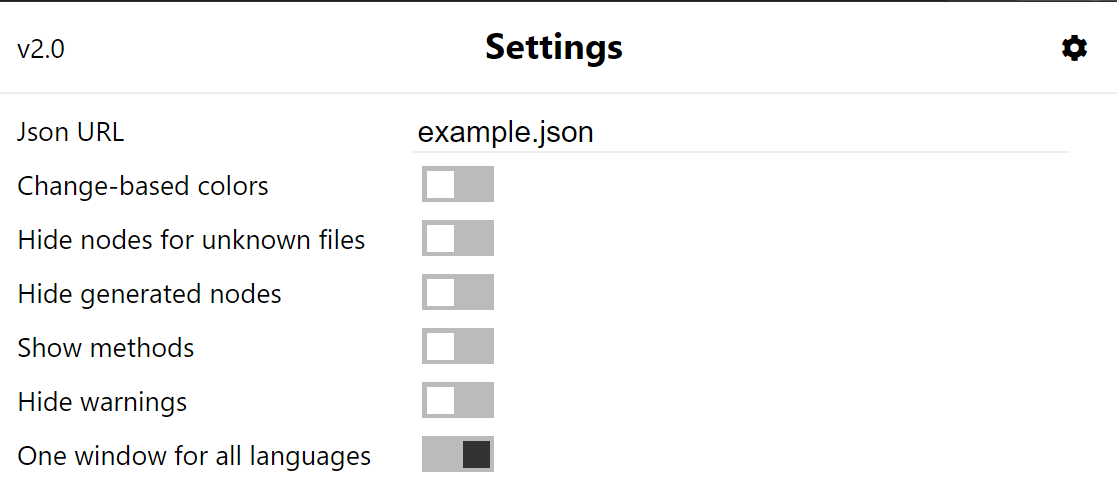
\includegraphics[width=0.8\textwidth]{Subfigures/settings.PNG}
    \caption{Settings for the tool exposed to the user. They can be adjusted within the browser.}
    \label{fig:CDVSettings}
\end{figure}


\subsubsection{Interactions} \label{SubSubSec:FrontendInteractions}
There are multiple ways to interact with the graph to help the reviewer adjust it to their needs, navigate within it, and navigate between it and the code under review. Most interactions, including navigating between the graph and the code and adjusting the graph layout, are similar in functionality to the ones described by Fröhlich \cite{publication-20661}, therefore we only repeat the most important ones here: The appearance of the graph can be changed by moving the nodes around. By hovering over a node, users can highlight the parts of the graph that are connected to it. Users can navigate between the graph and the code by clicking on a node to jump to the relevant code in GitLab (graph-to-code) and hover over code in GitLab to highlight the corresponding node (code-to-graph). Finally, nodes can be removed completely by right-clicking them.

A new way of customizing the graph was implemented for combining graphs of multiple languages into one graph. This removes the need for multiple windows which have to be managed separately, but moves the problem of managing the graphs into one window. Displaying multiple graphs takes up screen space, and developers might only be interested in a subset of the graphs. To combat this, each languages’ graph’s visibility can be toggled individually within the containing window, with nodes having a colored border indicating their language. Figure \ref{fig:MultiLanguageExample} shows part of such a graph and the language toggles. This way reviewers can adjust the graphs to their needs, while preserving the advantages of having only one window.

\begin{figure}[h]
    \centering
    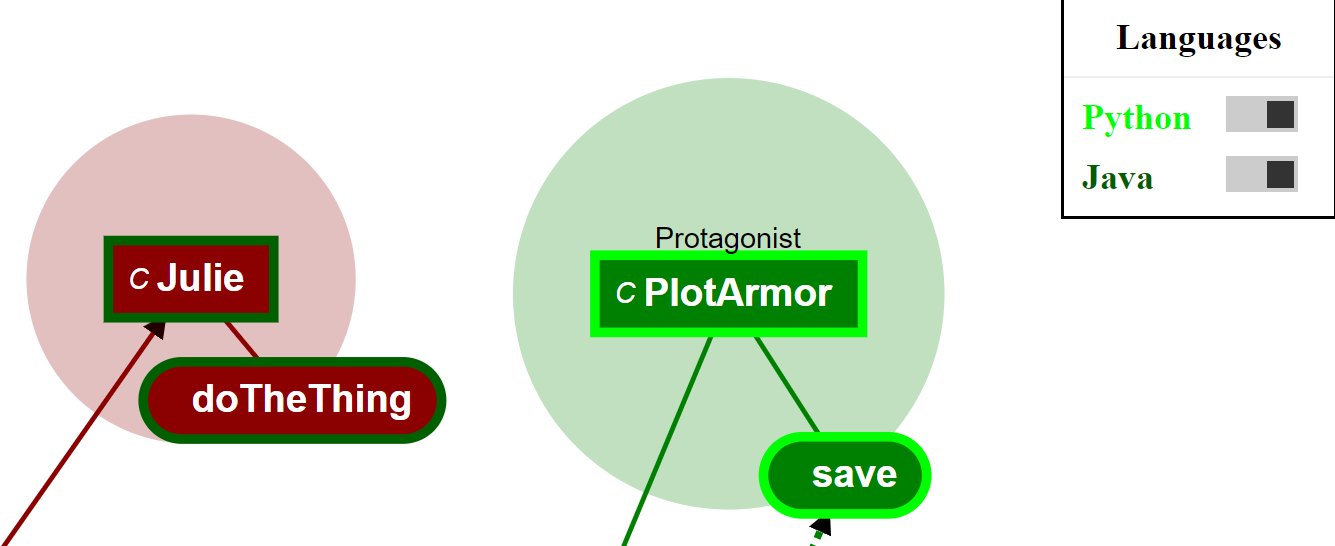
\includegraphics[width=1.0\textwidth]{Subfigures/multi_language_snippet.PNG}
    \caption{Snippet from a graph containing multiple languages, with one node for each language.}
    \label{fig:MultiLanguageExample}
\end{figure}

Another addition is the added information for warning nodes. Warning nodes have a question mark in their corner, which can be clicked to bring up the warning information. For this, a new field is displayed in the top left of the window, listing all warnings the tool encountered in the file of this node. It can be closed again using the close button. Figure \ref{fig:WarningWindow} shows an example.

\begin{figure}[h]
    \centering
    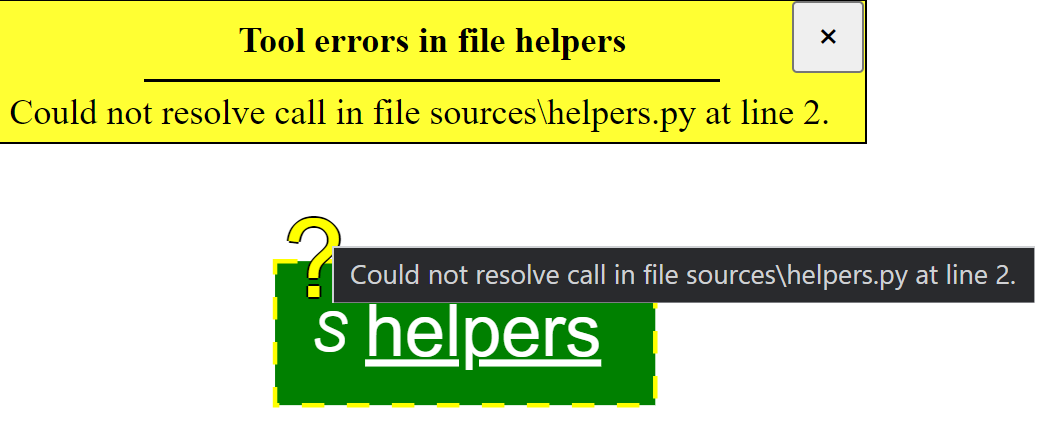
\includegraphics[width=0.8\textwidth]{Subfigures/warnings_window.PNG}
    \caption{Warning node with hover text, and the opened warning window.}
    \label{fig:WarningWindow}
\end{figure}


\subsubsection{A ReviewVis Example} \label{SubSubSec:ReviewVisExample}

To help explain the tool, we present a sample merge request and the graph created for it in Figure \ref{fig:CodeReviewExample}. It consists of four files, containing two classes, multiple functions, and some code not contained in any code entity. The change-based coloring is used, meaning deleted nodes are red, changed nodes orange, and added nodes green.

We further explain the graph using the numbers we added to identify specific elements:
 \begin{enumerate}
     \item Rectangular nodes with circles around them represent classes. They contain a C (for class) and the class name.
     \item Nested nodes have the name of the parent node displayed above them. Furthermore, a solid line with an arrow pointing towards the parent node links the node to its parent.
     \item Method nodes have rounded corners and are placed within the class circle. They contain the method name. A solid line connects them to their class node.
     \item Script nodes are displayed similar to class nodes (as they are root nodes as well). They contain an S (for script) and the filename.
     \item Dotted lines represent calls (both to methods and functions). They connect the calling node with the called node, with an arrow pointing towards the called node.
     \item Rectangular nodes without circle are class nodes. They contain an F (for function) and the function name.
     \item Functions can be nested, similar to classes. If they also get called by the parent node, only the calling relation is shown. The parent is still identified by the text above the node.
     \item Nodes can be disconnected from the rest of the graph, if they do not interact (in the code).
     \item A comment in GitLab is indicated by a blue C (for comment) on the node in which the commented line is. Hovering over it shows the comment(s).
     \item Tool warnings are displayed with a dotted yellow border and a question mark. The warnings can be displayed individually, or grouped together on a per-file basis.
 \end{enumerate}

\begin{figure}
\centering
\begin{subfigure}{.5\textwidth}
  \centering
  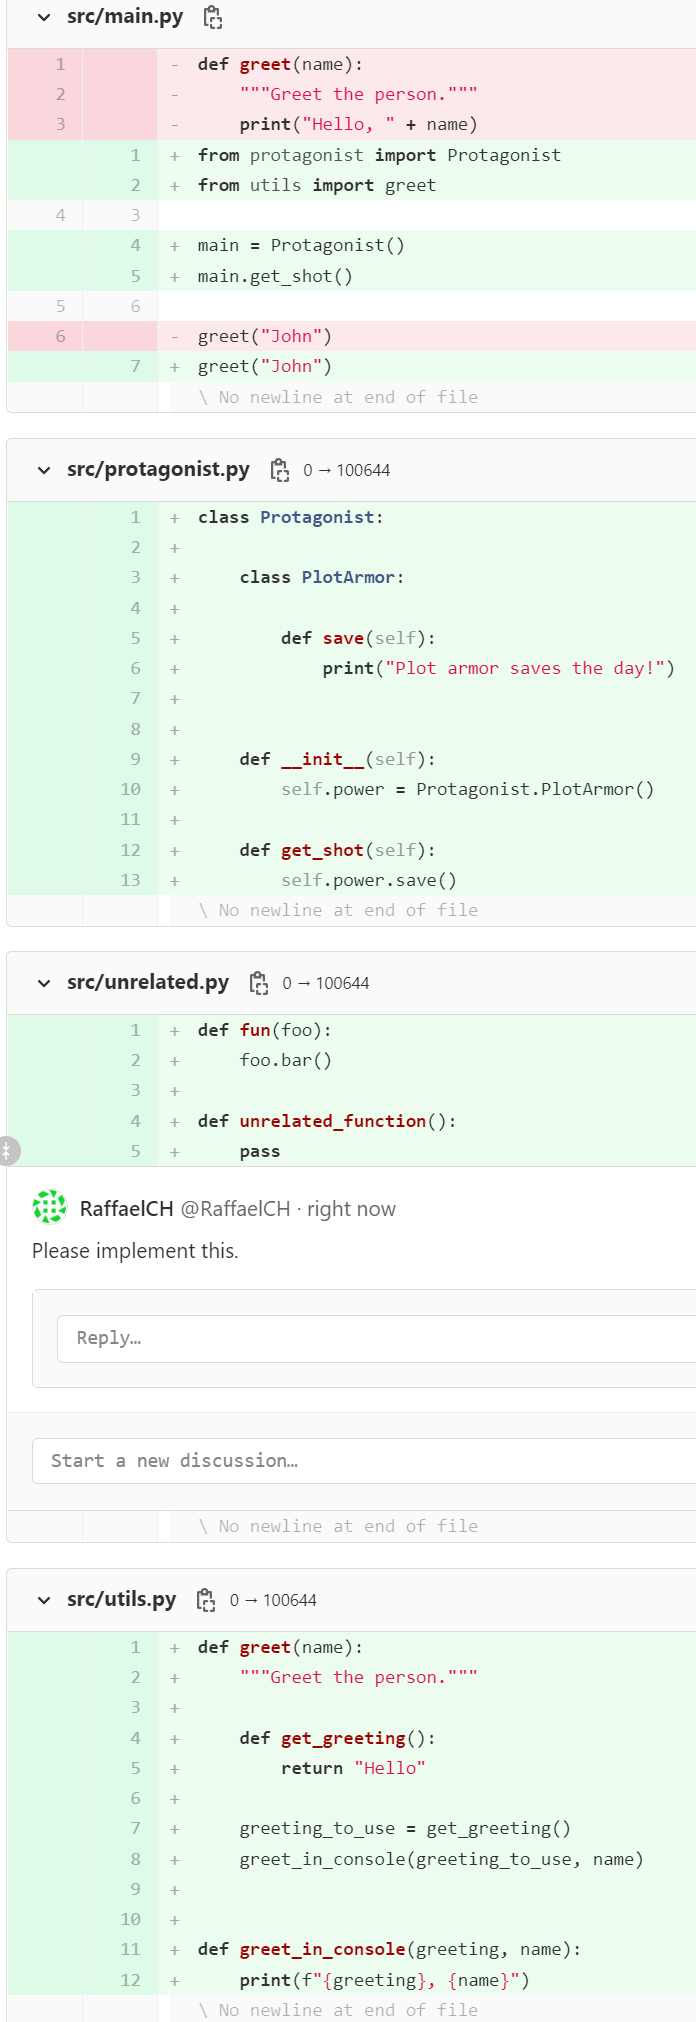
\includegraphics[width=1.0\linewidth]{Subfigures/gitlab_example_code.PNG}
  \caption{GitLab merge request.}
  \label{fig:GitLabExample}
\end{subfigure}%
\begin{subfigure}{.5\textwidth}
  \centering
  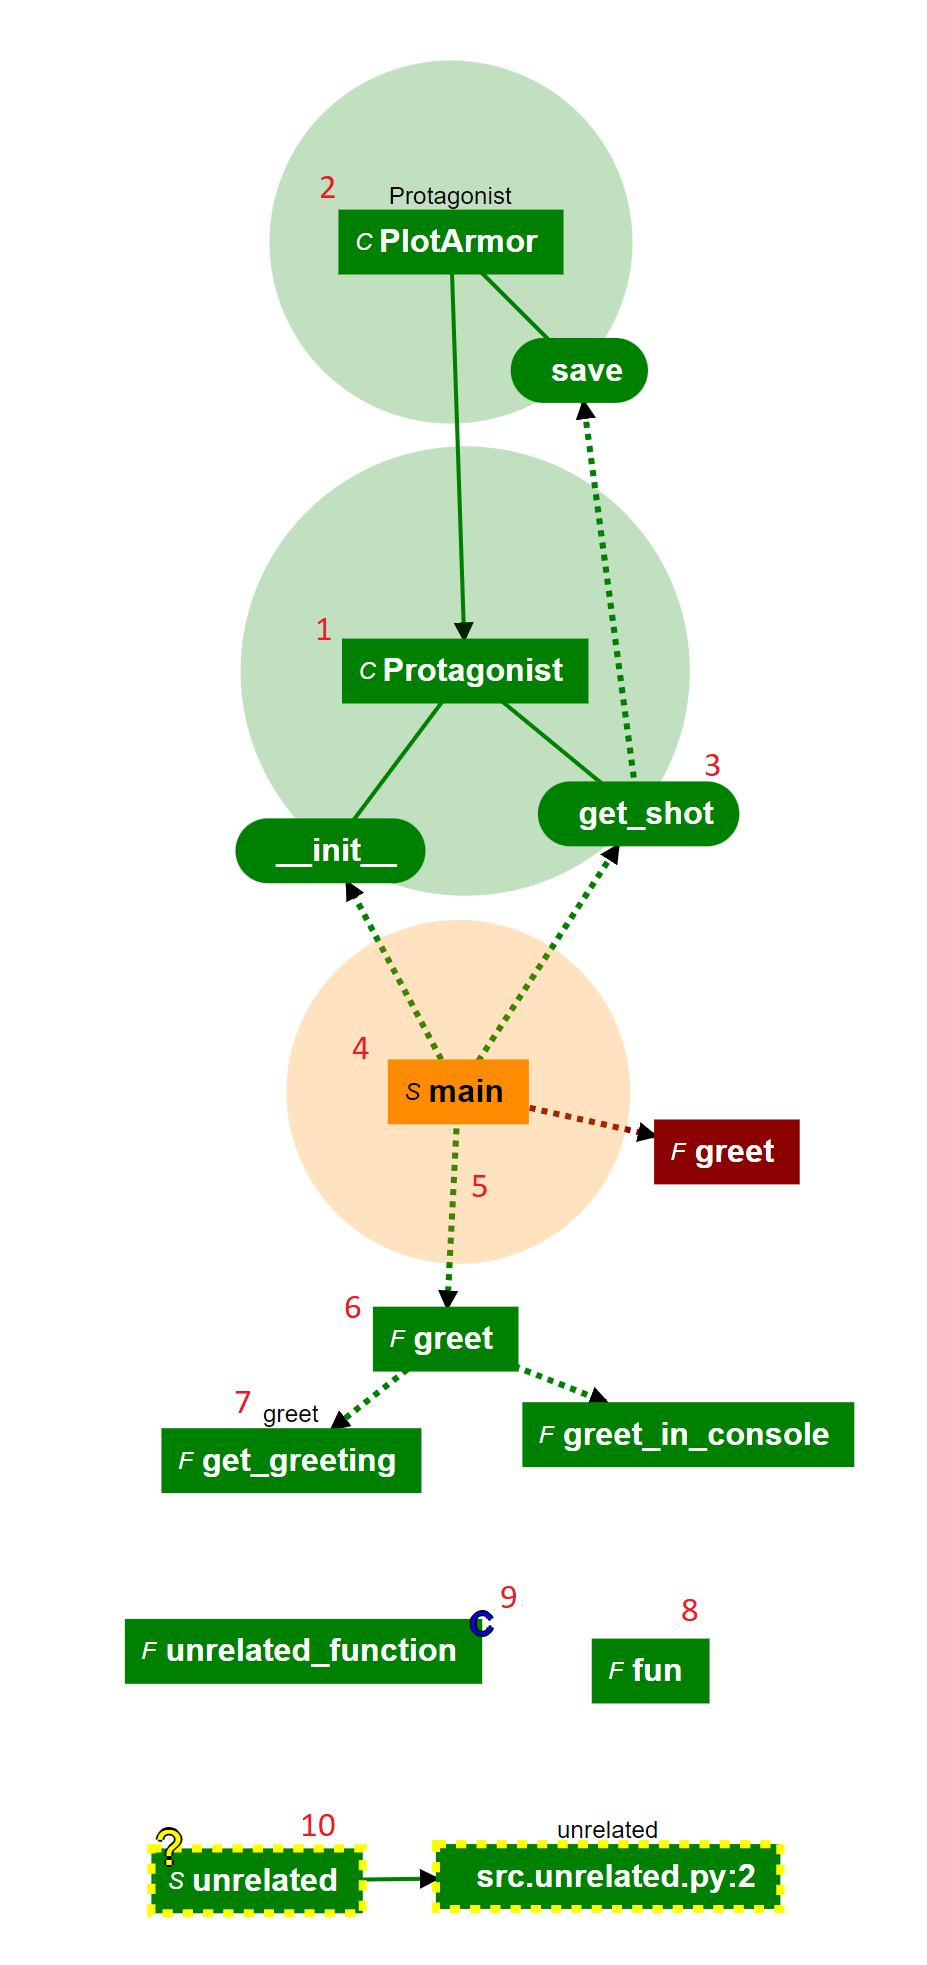
\includegraphics[width=1.0\linewidth]{Subfigures/annotated_example_graph.png}
  \caption{Graph created for GitLab merge request.}
  \label{fig:ReviewVisExample}
\end{subfigure}
\caption{Merge request with corresponding graph showing different aspects of the tool. GitLabs diff-based code view is on the left, and the created graph with annotations on the right.}
\label{fig:CodeReviewExample}
\end{figure}


\newpage


\section{Research Questions} \label{Sec:ResearchQuestions}
The principal goal of this thesis is to extend the ReviewVis tool to support multiple programming languages, as previous research found this to be one of the primary limitations of the tool\citep{publication-20661, cr_visualization_major}. We chose Python on account of it being a popular programming language, ranking in the top 3 in the TIOBE index\footnote{https://www.tiobe.com/tiobe-index/}, the RedMonk programming language rankings\footnote{https://redmonk.com/sogrady/2022/03/28/language-rankings-1-22/} and IEEE Spectrum\footnote{https://spectrum.ieee.org/top-programming-languages-2021}. Additionally, it also supports functional programming, in contrast with Java which is heavily OOP oriented, which allows us to evaluate graph-based code visualizations for functional programming paradigms. We implemented the backend in Python to extract the graph, and extended the frontend to support visualizations in Python (and other functional programming languages). Support for reviewing multiple graphs in different languages was also added. To evaluate the tool's extension, ReviewVis was shown to developers in a series of interviews to discuss our implementation. To better understand developers needs and inform future work on the tool, we also explored in these interviews how the existing work could be improved, and what features could be added to better support developers during code review. We aimed to answer the following questions:
\\

\fbox{\begin{minipage}{13cm}
\textbf{RQ1.1} What is a reviewer’s perception of ReviewVis when applied to merge-requests containing only Python code?
\end{minipage}}
\\

The goal of RQ1.1 is to evaluate the tool for Python, which supports both object-oriented and functional programming language paradigms. We compare it to GitLabs file-based diff view. As such we can evaluate the tool for Python specifically, while also evaluating our approach for different programming paradigms at the same time, including the newly added functional programming. This is done by conducting a series of interviews, showing developers the tool in multiple examples and asking their opinion, as well as collecting their feedback in a questionnaire.
\\

\fbox{\begin{minipage}{13cm}
\textbf{RQ1.2} What is a reviewer’s perception of ReviewVis when applied to merge-requests containing both Java and Python files?
\end{minipage}}
\\

RQ1.2 evaluates the tool’s performance when performing a code review for multiple languages concurrently. This is done by having a sample code review combining Java and Python, and iterating over developed solutions for displaying multiple graphs concurrently. The evaluation is done like for RQ1.1.
\\

\fbox{\begin{minipage}{13cm}
\textbf{RQ2} How can ReviewVis better support developers during code review?
\end{minipage}}
\\

RQ2 aims to understand the limitations of ReviewVis in its current form, and what the most important potential improvements and features for the tool are to guide future work. To find out, in addition to evaluating the tool to identify limitations based on research questions 1.1 and 1.2, the interviews were also used to collect and discuss ideas for new features. Some of them are implemented between interviews in accordance with the RITE methodology to enable collecting of feedback and further development during the following interviews.

\newpage


\section{Evaluation} \label{Sec:Evaluation}

In this chapter, we go over the RITE methodology we used and how we adapted it, and the interviews and online questionnaire for evaluating the tool. After that we answer the research questions, ordered by subtopic where needed.


\subsection{Methodology} \label{SubSec:Methodology}
For the evaluation, we collected feedback from developers using the RITE methodology, with improvements being made to the tool between interviews. We describe the methodology used and our justification for it in sections \ref{SubSubSec:RITE} and \ref{SubSubSec:RiteAdaptations}. We go over the interview structure in section \ref{SubSubSec:RiteIterations}.

\subsubsection{Rapid Iterative Testing and Evaluation (RITE)} \label{SubSubSec:RITE}

The Rapid Iterative Testing and Evaluation method (RITE) can be used to quickly identify issues and fix them, before verifying the effectiveness of the changes. It has first been formally introduced by Medlock et al. when it was applied to identify and fix issues in a game tutorial in 2002 \cite{Medlock2007UsingTR}. In their study, issues found during each iteration were discussed, before being fixed. Each new version was then retested. In each iteration the number of issues encountered were counted, and the study was continued until five consecutive participants encountered no issues. 

One of RITE’s advantage over more traditional usability evaluations is that any changes that were applied can be rechecked, helping in discovering issues that need to be further improved. By iteratively adapting, the same features can be tested more often with different user interfaces. 

Since then, the methodology has been adapted by researchers to better fit their needs. One is to conclude the study sooner. This is done to save costs, and it relies on the concept that major issues are often found in the earlier iterations \cite{6606617, Rong2012TheEO}. 


\subsubsection{RITE Adaptions} \label{SubSubSec:RiteAdaptations}

In the interviews we used a holistic approach, where we evaluated all aspects of the tool. In accordance with RITE, graphical improvements and simple to implement features were directly implemented in the next version of the tool, so they could be evaluated in practice and iterated upon if necessary. For more complex changes and advanced features, a possible outline for an implementation was presented. Participants were asked to give feedback, and possible approaches were discussed. This allowed for the rapid introduction and evaluation of new features and ideas, further improving the tool in the scope of this thesis as well as collecting data for future work. 

Originally the RITE methodology did not limit the number of iterations but continued until enough consecutive evaluations returned no issues. While this can be a feasible approach when designing a user interface, in the context of developing new features as well as collecting and evaluating ideas this is not possible due to the open-ended nature of the process. We argue that this is especially true for more experienced users, who are going to have more ideas about the process and how and what a tool should do. 

To adapt to this, we used an approach where the number of evaluations is predefined to limit the length of the study, which is also used in other studies and industry \citep{10.1145/2858036.2858387, rite-way-to-prototype, really-ingenious-testing-experience}. A follow-up study is used to further test the tool at this state to counterbalance the adaption of the methodology. Fregnan et al. found that an iterative approach with a limited number of users was a good compromise between limiting the length of the study and collecting enough feedback \cite{Fregnan2022}. We argue that this is also true for this study, and that a limited evaluation run with a final feedback run produces sufficient data for our purposes of evaluating the tool and exploring opportunities for future work. 


\subsubsection{RITE Iterations} \label{SubSubSec:RiteIterations}

The evaluations were done remotely via a video call using Zoom\footnote{https://zoom.us/}. Doing it remotely allowed for greater flexibility regarding who could participate and when. The interviewer showed to the participants demos of the tool running on their machine for a set of publicly accessible merge requests, with the screen being shown to the participants. Participants could indicate parts of the tool to talk about and ask for features and actions to be demonstrated. 

At the beginning of the interviews, an introductory question about code review was asked to establish working experience and tools usage (a more detailed survey was done in a follow-up questionnaire). After that, a quick overview over the tool and its aim was given. 

All examples were presented by having one window with the code under review in a merge request on GitLab, and another window containing the corresponding graph. These windows were positioned side-by-side on the same screen, so everything was visible at the same time. For the largest example with multiple graphs, the graph was shown in full screen for some time when initially presented to the developer. 

For evaluation purposes three scenarios were presented to the participants: a small code change in Python only involving code entities, a bigger change with a more complex graph including non-Python files and tool errors, and a final scenario involving both Java and Python code changes. Pictures of the graphs can be found in Appendix \ref{App:InterviewExampleGraphs}. The scenarios were presented in increasing complexity, with some interactions and features being presented only in the second example. This was done to give participants the opportunity to get used to the tool and understand it before being confronted with the more complex graphs. Short explanations were given for the graph, interactions and settings, and participants were allowed to ask questions if they felt they did not understand something. We argue that by the end of the interview the participants had a sufficient understanding of the tool to give useful feedback and estimate the long-term usefulness of the tool. 

Each RITE iteration was structured as an interview, where we asked participants open questions about different aspects of the tool. The most important was the graph visualizations and way of displaying node types for multiple different graphs, asking them about the general impression and usefulness of it, as well as hurdles to adoption and issues. As the settings could modify the graph, they were evaluated by comparing the graphs with and without them on, when applicable. The interactions were usually evaluated after introducing the graph itself, but when participants brought them up earlier, discussions were started before explaining all details of the graph. Finally, the last example evaluated the tool for multiple languages, showing different settings and asking about ideas on how to solve it. A scheme of the interviews structure is available in Appendix \ref{App:InterviewStructure}. These were used to start the conversation and as a guideline. They were extended by questions about specific issues, features and ideas for possible improvements collected over previous interviews. As the interviews progressed and areas of special interest were identified as well as more ideas collected, more space was given to less structured conversations about these ideas to maximize new insights. 

In each interview after the first, extra space was given to the changes introduced since the last interview. This was to properly evaluate the changes made and new features introduced, and further iterate on them if necessary. For more impactful changes, versions with and without these changes were shown to the participants, and they were asked what their opinion was. 

Most interviews lasted for around 40 minutes with some taking over an hour, depending on the participant and their ideas and available time. As more information was collected over the interviews, the average time increased because more previously collected insights could be discussed. 


\subsubsection{Post-interview Questionnaire} \label{SubSubSec:Questionnaire}

After the interviews, participants were given a link to a short (about 10 minutes to fill out) online questionnaire, available in Appendix \ref{App:Questionnaire}. In it we used the Technology Acceptance Model \cite{davis-1989} to assess the participants perceptions of the interface. It is a model to assess the user's perception of a technology’s usefulness and its ease of use to predict the user's acceptance. The three main questions of TAM, perceived usefulness, ease of use and self-predicted future use, were measured. To measure the participant’s agreement with each statement, a 5-point Likert scale was used, ranging from “Strongly Disagree” to “Strongly Agree”. We also collected demographic information and previous experience in this questionnaire. The responses were linked to the interviews by a code given to the participants. 


\subsubsection{Demographics} \label{SubSubSec:Demographics}

\begin{table}[h!]
\begin{center}
\begin{tabular}{ m{1cm} | m{1.5cm} |  m{3.5cm} | m{2cm} | m{2cm} | m{2cm} } 
 \rowcolor{lightgray} ID & Male & Current Occupation & Professional Coding Experience & Professional Python Coding Experience & Prof. Code Review Experience \\
 \hline
 P1 & Male & Software Developer, Engineering Manager & 6-10 & 3-5 & 6-10 \\
 
 P2 & Male & Software Developer & 11+ & 3-5 & 11+ \\
 
 P3 & Male & Student & 2 & 2 & 1 \\
 
 P4 & Male & Student & 1 & 1 & 1 \\
 
 P5 & Male & Software Developer & 11+ & 0 & 6-10 \\
 
 P6 & Male & Software Developer & 11+ & 0 & 11+ \\
 
 P7 & Male & Software Developer & 11+ & 1 & 11+ \\
 
 P8 & Female & Student, Researcher & 3-5 & 0 & 2 \\
\end{tabular}
\end{center}
\caption{Overview of the participants ordered by interview date.}
\label{table:ParticipantsOverview}
\end{table}

The interviews were conducted with eight participants, listed in Table \ref{table:ParticipantsOverview}. Seven were male and one female. Five were working as software developers with one also being an engineering manager, and three were students with one also being a researcher. 62.5\% of the participants programmed daily and did code review at least once a week. Four of the interviewees have developed software professionally for over 10 years, two for more than 3 years, and two for 2 years or less. Five participants had at least 6 years of code review experience, with the others having 2 years or less. Participants had less experience with Python, with only three participants having over 2 years of experience and three participants having no experience at all.


\subsection{Results and Analysis} \label{SubSec:ResultsAnalysis}

Here we present the results of the interviews and the follow-up questionnaire. First, we give an overview over the demographics, before answering the research questions. We used an outline for the interviews to guide the discussion. Furthermore, developers provided new suggestions and ideas to improve ReviewVis, going beyond the predefined questions. We categorized the results where possible to structure the large amount of information collected in the interviews.


\subsubsection{Developer’s Perception of ReviewVis With Python} \label{SubSubSec:RQ1.1}

\paragraph{General Perception of ReviewVis} \label{Par:OverallImpressions}
The primary benefit of ReviewVis as identified by developers in the interviews was giving an overview of the code changes themselves (7 out of 8 developers) and to see the context of the code changes made (4 out of 8 developers). The overall perception was positive with most developers describing the tool as useful or helpful, and five of them expressing that they want to try it out or use it in their code reviews. Similarly, in the questionnaire all except P5 (who criticised the default node positioning) predicted that they would use ReviewVis in the future, and all participants answered that they preferred it over only using GitLab.

\begin{figure}[h]
    \centering
    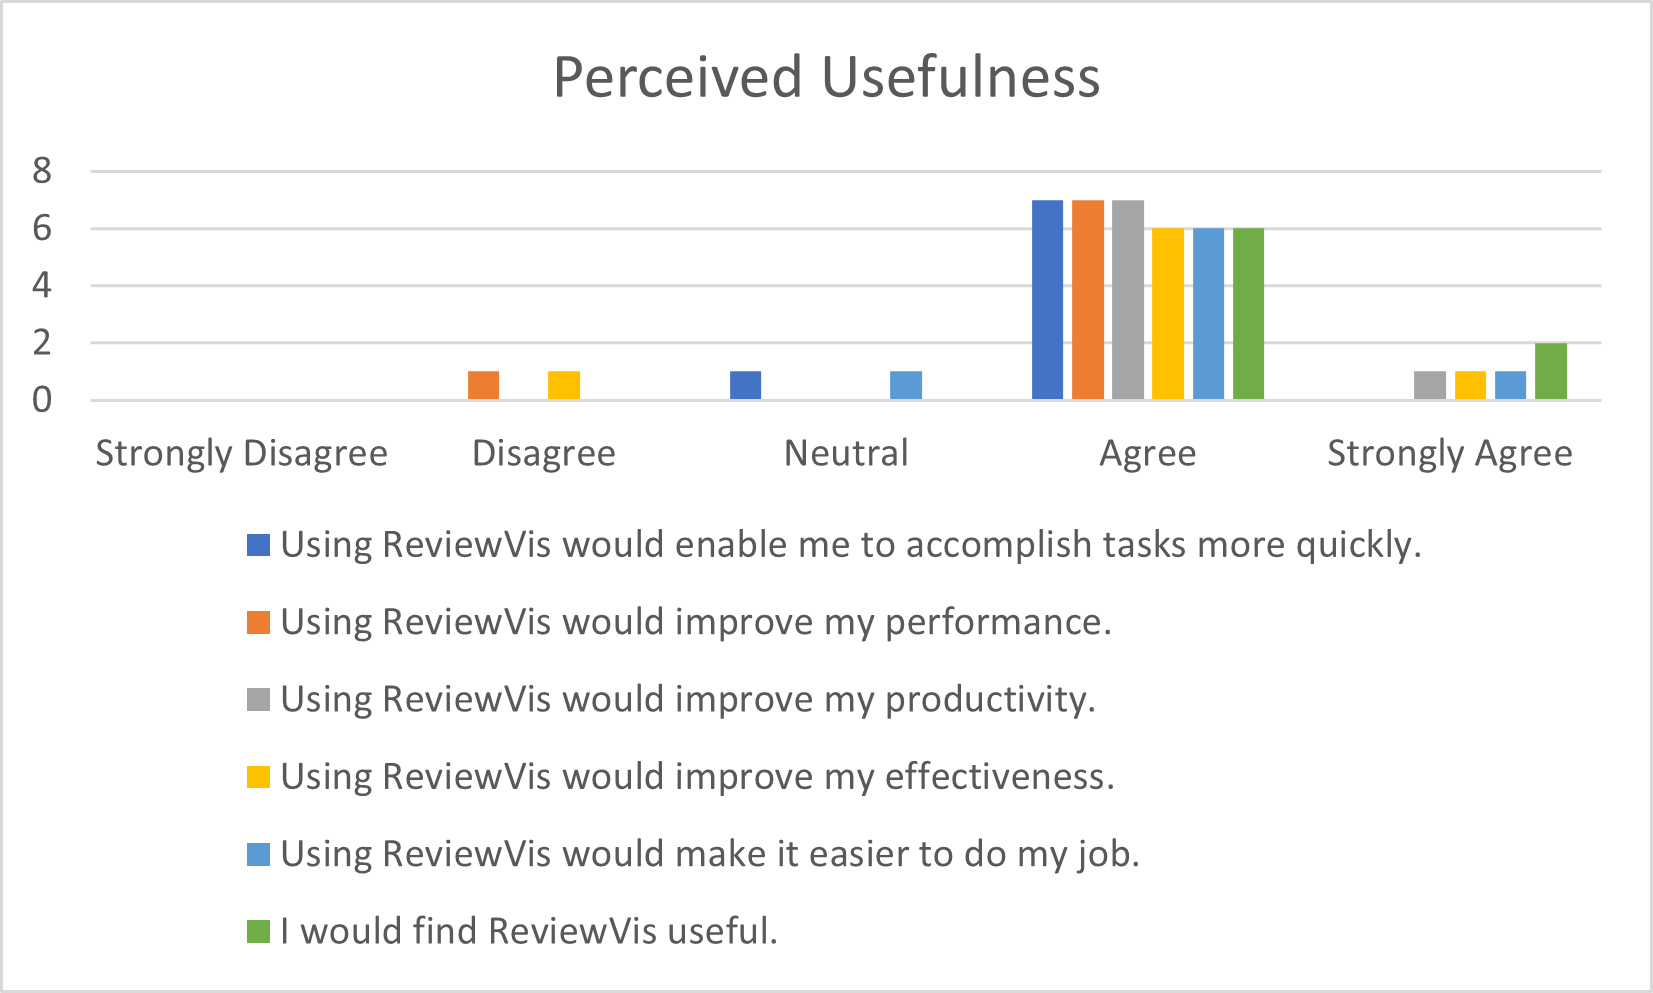
\includegraphics[width=1.0\textwidth]{Subfigures/perceived_usefulness.png}
    \caption{Usefulness of ReviewVis as perceived by the participants.}
    \label{fig:PerceivedUsefulness}
\end{figure}

When asked about the usefulness of ReviewVis in the questionnaire, participants' answers were mostly positive: all participants answered that they think ReviewVis is useful and that it would increase their productivity. Participants were unsure if the tool would improve their performance and effectiveness, with P1 thinking it would hinder him in both. Participant P5 was not sure whether the tool would speed up their work and answered that it might not make their job easier. The answers are summarized in Figure \ref{fig:PerceivedUsefulness}.

The usefulness of the tool depends on the size of the review changeset. For smaller changesets, where only a few nodes are touched, the resulting graph is relatively small. For these cases developers expected the tool to be less useful, as they would be able to quickly understand the changeset without the tool. Some developers with over a decade of experience expressed that for more mature or well-organized code bases, most changes can be made locally (i.e., without touching a lot of nodes) and as such the tool would not be needed often. But for large changesets ReviewVis becomes useful, since these changes are the most complex and therefore the hardest to understand (according to developers). For instance, a participant mentioned large-scale refactoring as a case where our tool would be beneficial, showing the overarching pattern of the change. 

Another factor that impacts the usefulness of the tool is the complexity of the graph, as measured by the number of nodes and relations. In its current form, most developers thought that ReviewVis provides an appropriate level of abstraction by default. Potential problems they mentioned were extremely large numbers of nodes or densely connected graphs. When evaluated for a graph with over 20 connected nodes and nearly 40 relations between them, the feedback was still positive but more mixed: Two participants thought the graph was too complicated, while four thought that it still was useful, especially with the ability to highlight specific parts of the graph. When asked about the setting to hide methods and therefore reduce the graph complexity, developers reported it as not useful unless the graph becomes too complex. Participants reported that for the examples used (12-34 nodes with 10-54 connections), the level of detail is appropriate. The tool was not evaluated for graphs containing more than 34 nodes. Participant P2 thought the tool would even be useful for reverse engineering, which could involve graphs spanning hundreds or thousands of nodes. Two developers answered that the tool could be useful for understanding even very large graphs, although we expect this to heavily depend on the exact structure of the code change. 

Another benefit of the tool that P7 brought up is that it can quickly indicate how something was implemented. Using the graph, reviewers can see if an existing class was modified, a new one added, and what classes or functions were changed. They thought this could make the tool helpful for automatically creating the graph and displaying a picture of it in another tool alongside other information. Specifically, they thought of Jira\footnote{https://www.atlassian.com/software/jira}, an issue tracking platform. The example they gave was that there could be a task to review a modification. When this task is created, an automatic process creates a picture of the visualization and links it to the task, where it is shown together with it. The reviewer could then with one glance see what was done, without having to leave the platform. Another benefit of this approach that they mentioned is that more users get exposed to the tool, potentially convincing them to try it out.

In some cases there can be nodes that are (visually) not connected to the other nodes: e.g., when a function is added which does not interact with other code in the changeset, resulting in it not being connected to the rest of the graph. Two participants said that they were confused by them. But our tool only displays the structure of the code. If a developer creates a merge request resulting in such a situation, e.g. by combining multiple disconnected changes into one merge request, the tool will just display the result. Therefore this is a situation that is inherent to our approach, but we think that explaining how this can occur will be enough to prevent confusion.

An important problem of the tool, especially for large and complex changes, is the initial positioning of the nodes in the graph. Currently the main nodes like class, function and script nodes are positioned randomly in a circle, with method nodes being positioned around the class nodes. This does not take the interconnections between nodes into account, which can lead to suboptimal placements with lines crossing each other. The use of different forces between the nodes then pulls them into the final configuration which improves the positioning but does not solve the problem. This was criticized by half of the developers.

To address this, an algorithm to position the method nodes closer to nodes connected to them was implemented: Instead of spreading them out randomly around the class node, the connected nodes for each method are collected. For each connected node, the angular position is calculated as a vector of length 1, pointing from the class node to the connected node. These vectors are then added and normalized to obtain the methods angular position as a vector. The direction of the vector gives the direction in which the method node should be positioned, relative to the class node. The length of the vector encodes the priority (i.e., longer vectors mean that this method's connections are less spread out, and therefore it is more important to position them at their position). Then, the methods are positioned around the class node, with longer vectors being prioritized. If this position would result in being too close to an already positioned method, the angular direction is adjusted until it is far enough away from other methods (minimum distance decreases in number of methods). This way, if the connections are more spread out, the method is positioned more flexibly. The outcome is that methods are positioned close to their connected nodes relative to the class. Figure \ref{fig:MethodPositioning} shows the procedure.

This improves the graph clarity especially for smaller graphs. But for large graphs with a lot of class nodes, positioning remains a problem. Manually dragging around the nodes to improve the positioning is possible and was seen as an acceptable solution, but it means more work and hinders the usage of the tool for automatic graph creation. Good automatic positioning was seen as superior to manual positioning.

\begin{figure}[h]
\centering
\begin{subfigure}{.5\textwidth}
  \centering
  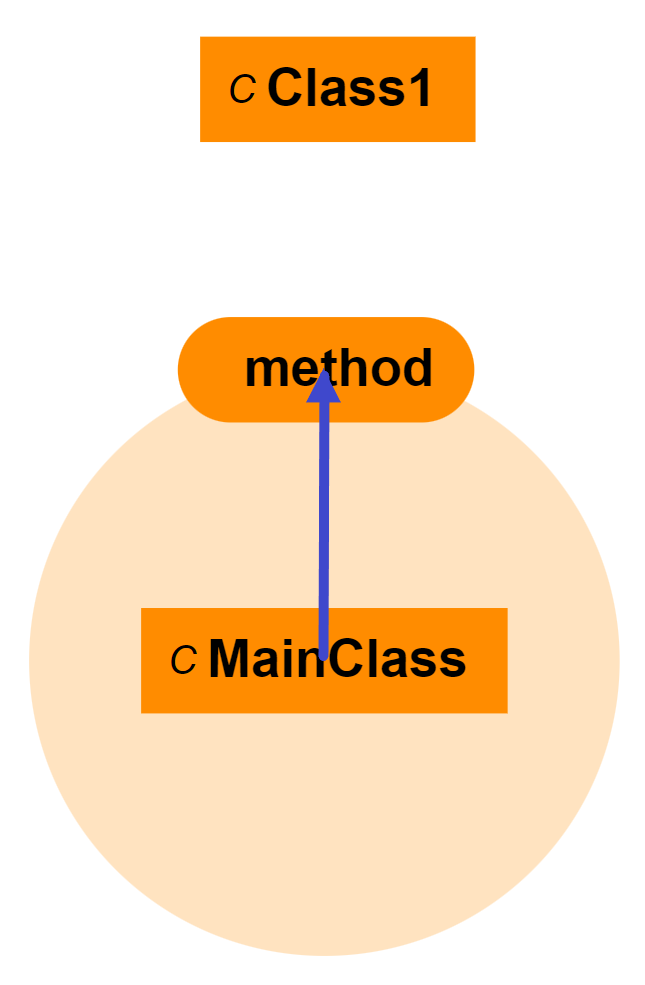
\includegraphics[width=0.5\linewidth]{Subfigures/method_positioning_example1.PNG}
  \caption{Only one connection.}
  \label{fig:MethodPositioning1}
\end{subfigure}%
\begin{subfigure}{.5\textwidth}
  \centering
  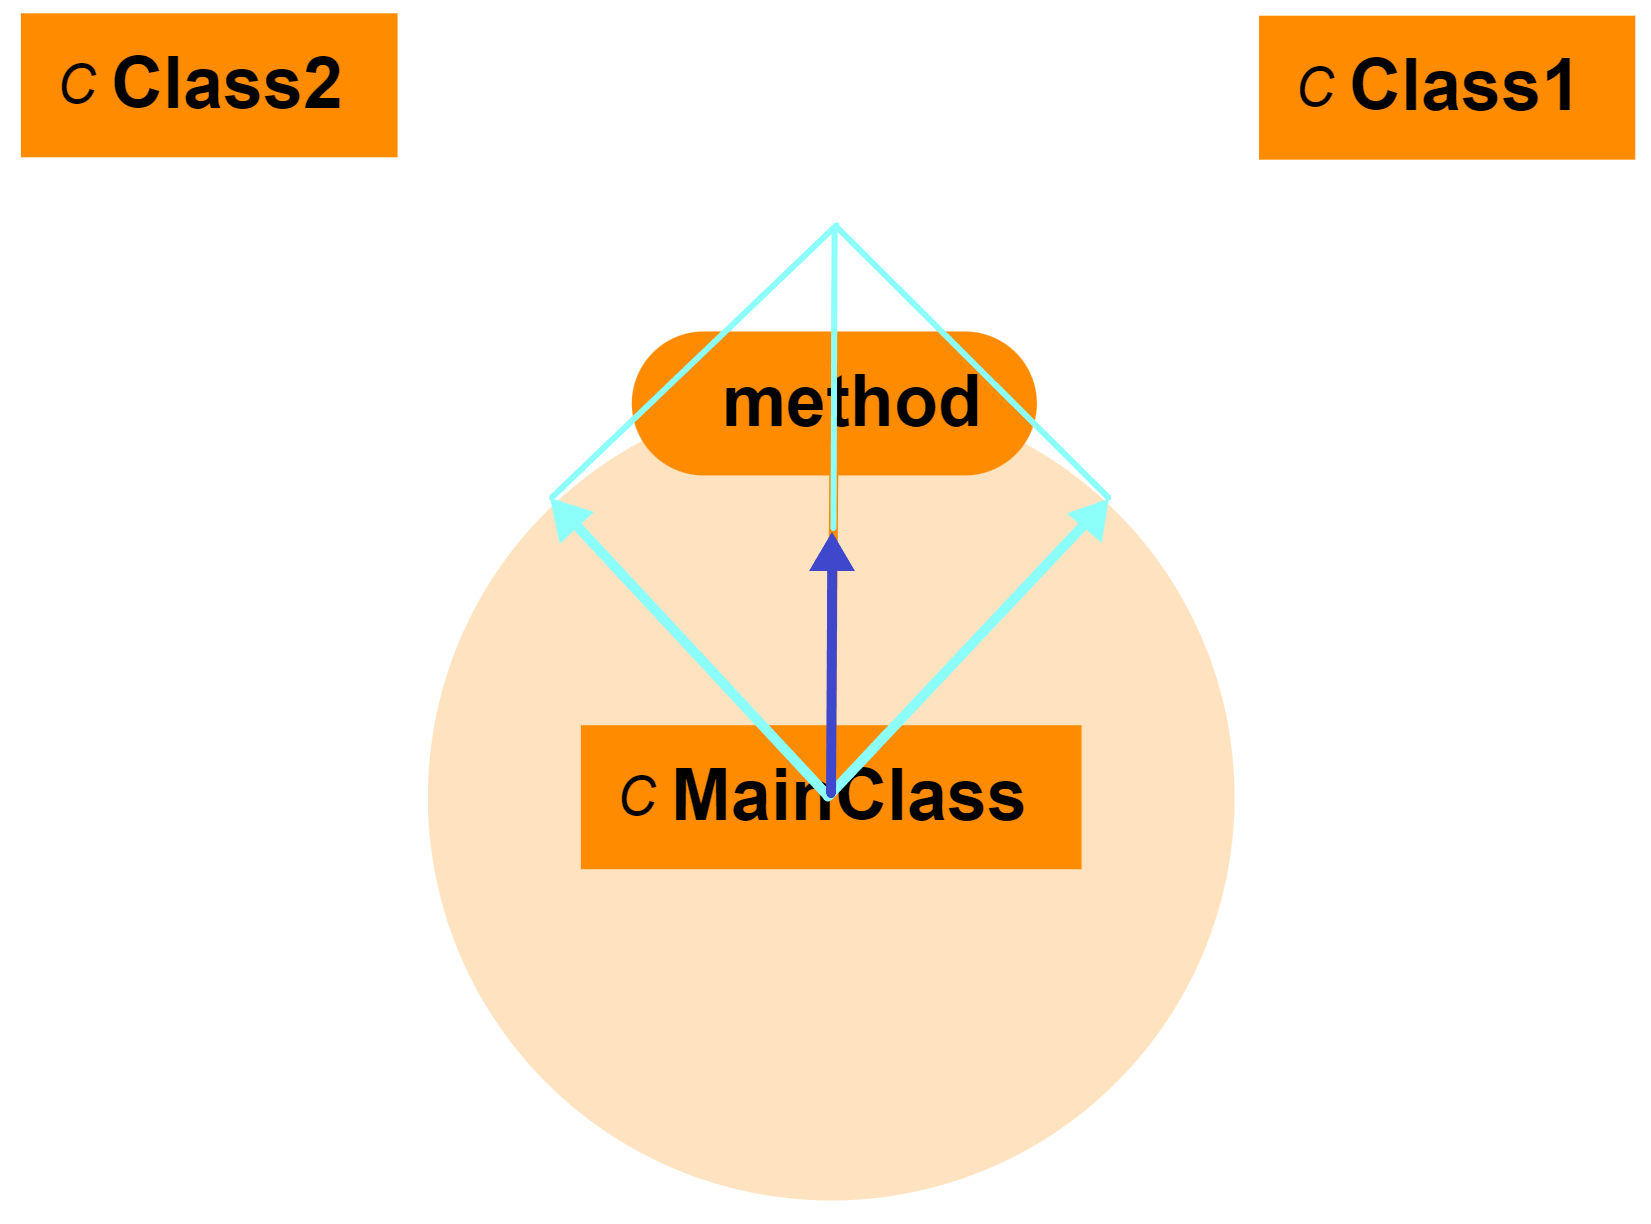
\includegraphics[width=1.0\linewidth]{Subfigures/method_positioning_example2.PNG}
  \caption{Two connections.}
  \label{fig:MethodPositioning2}
\end{subfigure}
\caption{A class node \textit{MainClass} with a method node \textit{method}. This method node is connected to other class nodes. In the left example, it is only connected to node \textit{Class1}, and the resulting angular position (blue arrow) points directly at the connected node. In the right example, the method is connected to two nodes, \textit{Class1} and \textit{Class2}. The resulting vectors are shown in light blue. They are summed up and normalized to obtain the vector for the final method position (dark blue arrow). The direction is between the two nodes, and the vector is shorter because the connections are more spread out.}
\label{fig:MethodPositioning}
\end{figure}


\paragraph{Graph Design and Features} \label{Par:GraphDesignFeatures}

Regarding the design of the graph, the participants thought that the way the nodes themselves are designed is good, and that indicating the type of node for similar-looking nodes (classes, functions, interfaces, etc.) is understandable after a few minutes. Three of the first five participants experienced confusion over the design of the relations: they said that method dependencies and calls looked too similar, with both being dotted lines just with different length of intervals (see Figure \ref{fig:links-initial} for an example). To address this problem, the relations between methods and their classes were redesigned to resemble dependencies, shown in Figure \ref{fig:links-final}. This reduced the number of relation designs to two clearly distinct types, and in later interviews this problem did not come up again. 

Other improvements made for the relations were the addition of arrows. While for some relations the meaning was clear (e.g., the connection between a class and a method), developers mentioned that for some relations like class dependencies, the direction is unclear from the graph alone (see Figure \ref{fig:links-initial} for an example). To communicate this information to the users, arrows were added to all relations except method dependencies, as in this case the relation type was already clear (see Figure \ref{fig:links-final} for the updated design). In subsequent interviews, participants either expressed no confusion anymore or even mentioned the arrows positively. 

\begin{figure}
\centering
\begin{subfigure}{.5\textwidth}
  \centering
  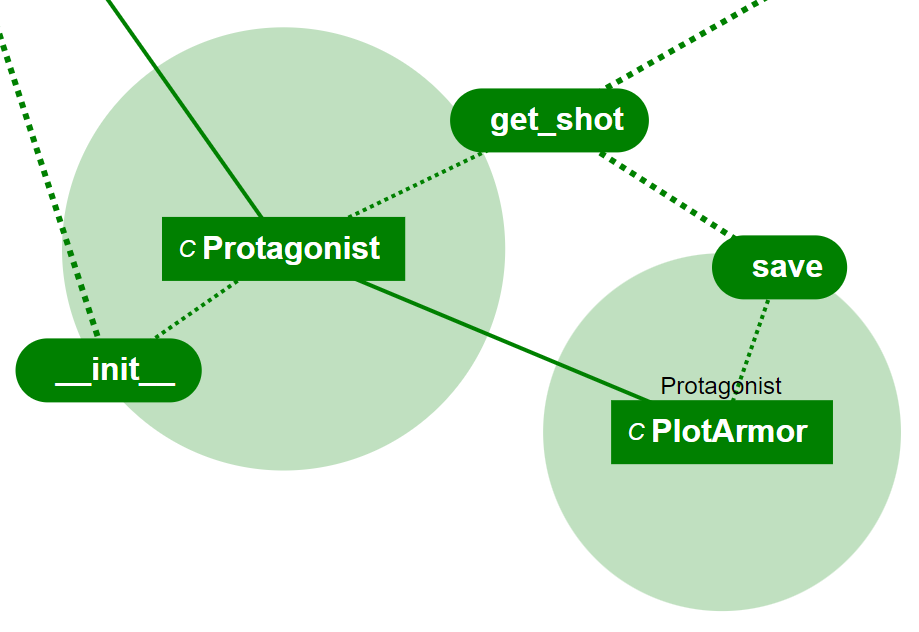
\includegraphics[width=0.9\linewidth]{Subfigures/links-initial.PNG}
  \caption{Before}
  \label{fig:links-initial}
\end{subfigure}%
\begin{subfigure}{.5\textwidth}
  \centering
  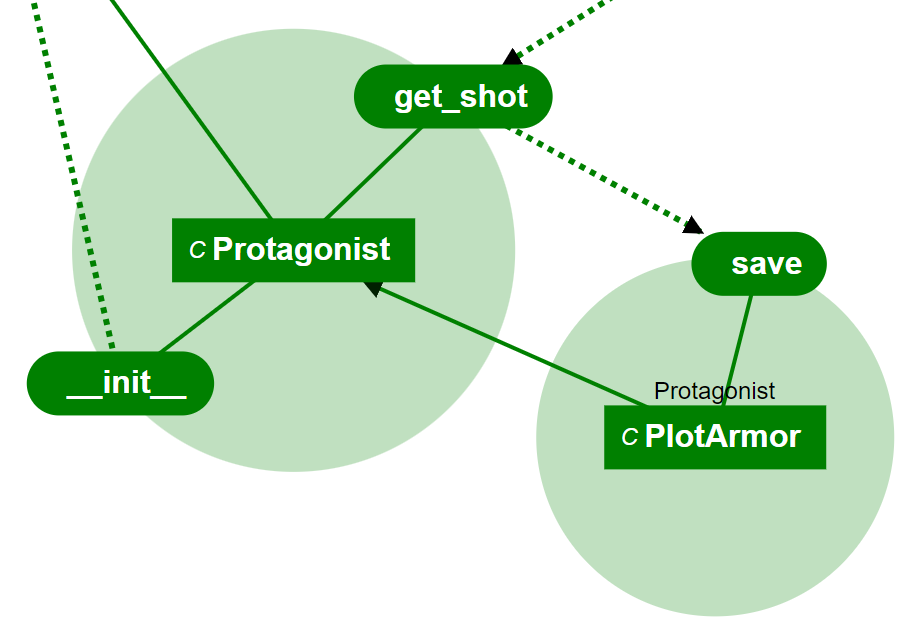
\includegraphics[width=0.9\linewidth]{Subfigures/links-final.PNG}
  \caption{After}
  \label{fig:links-final}
\end{subfigure}
\caption{Part of a graph showing a nested class (PlotArmor) and its parent class (Hero), with the method \textit{Hero.get\_shot} calling the method \textit{PlotArmor.save}. On the left is the initial link design, and on the right the final link design for the same links. Arrows were added and class-to-method links redesigned to make the relation types and directions clearer.}
\label{fig:linkComparison}
\end{figure}

In the graph, the parent node of nested classes and functions is indicated by the name of the parent node shown over the child node. In the case of nested functions, a function could be both the parent function and calling function, which would lead to two overlapping relations as shown in Figure \ref{fig:nested-function-links-initial}. This was confusing for some developers. We updated the graph to only show the calling relation, using the parent’s name to indicate the nesting (see Figure \ref{fig:nested-funtion-links-final}). When asked about this new implementation, developers answered that it’s not obvious but understandable and that they expect to get used to it. 

\begin{figure}[h]
\centering
\begin{subfigure}{.5\textwidth}
  \centering
  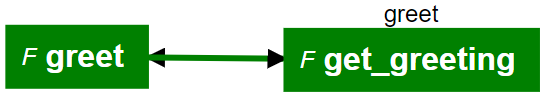
\includegraphics[width=0.9\linewidth]{Subfigures/nested_function_initial.PNG}
  \caption{Before}
  \label{fig:nested-function-links-initial}
\end{subfigure}%
\begin{subfigure}{.5\textwidth}
  \centering
  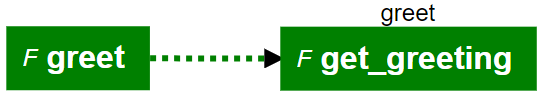
\includegraphics[width=0.9\linewidth]{Subfigures/nested_function_final.PNG}
  \caption{After}
  \label{fig:nested-funtion-links-final}
\end{subfigure}
\caption{Function \textit{greet} with a nested function \textit{get\_greeting}, which gets called by \textit{greet}. To prevent confusion, only the calling relation is shown with a link, with the parent relation being signified by the parent's name on top of the child node.}
\label{fig:nestedFunctionLinkComparison}
\end{figure}

The parser might not be able to retrieve all information in a review changeset (this is due to Python being a dynamic language using duck typing, see chapter \ref{SubSec:ModulesSymbolsPython} for a more detailed explanation). This needs to be communicated to the user so they know the graph might be incomplete. For this, warning nodes were added.

In their first iteration, warning nodes (or error nodes at this time) used a red exclamation mark to signify a (tool) error. As the exclamation mark was seen as too small, a checkered border was added after the first interview. Developers interpreted this as an error in the code and were confused. Errors within the tool were seen as less important than errors in the code, so the alarming messaging of the error node was thought to be a code error. In later iterations the colors were changed to yellow (communicating a warning) and a question mark instead of an exclamation mark to indicate the tool did not understand something. Figure \ref{fig:warningComparison} shows a comparison.

\begin{figure}[h!]
\centering
\begin{subfigure}{.5\textwidth}
  \centering
  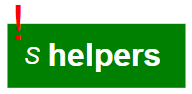
\includegraphics[width=0.3\linewidth]{Subfigures/warnings_initial.PNG}
  \caption{Initial warning node design.}
  \label{fig:initial-warnings}
\end{subfigure}%
\begin{subfigure}{.5\textwidth}
  \centering
  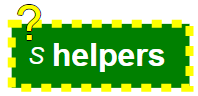
\includegraphics[width=0.3\linewidth]{Subfigures/warnings_final.PNG}
  \caption{Final warning node design.}
  \label{fig:final-warnings}
\end{subfigure}
\caption{Comparison of the initial and final (after the interviews) warning node design.}
\label{fig:warningComparison}
\end{figure}

This final design was received better by participants. At this stage, further information about the warning could be displayed by clicking on the question mark. Doing so opens a new window on the top right, which closes when the close button is pressed. Following feedback that the connection between the warning node and the window can get lost as the window stays open, the ability to show the warning information by hovering over the node was added. Participants in the subsequent iterations showed a (slight) preference for the hover text. However, hover text is only shown while hovering over the node, and moving the mouse closes it. For this reason, participant P8 would have preferred to additionally have a pop-up window like the existing one, but positioned in the middle of the screen while preventing the user from interacting with the graph until it’s closed.

A feature that was requested multiple times was showing which nodes were commented in GitLab, as code review is commonly done by commenting on the code. This way reviewers can pay more attention to these nodes. For this, comments are loaded when loading the GitLab page, and matched to the corresponding node in the graph. The node gets a blue C (blue because it has good contrast with the node colors, and C for comment), hovering over which displays all the comments and threads made on code belonging to this node. Figure \ref{fig:CommentIndicator} shows an example with multiple comments. When evaluated, the indicator (the blue C) needed to be explained initially, but after that they thought it is clear enough and that it is a useful feature. 

\begin{figure}[h!]
    \centering
    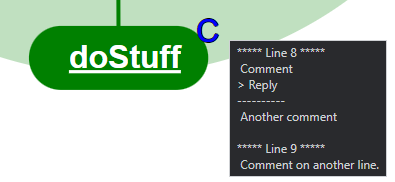
\includegraphics[width=0.5\textwidth]{Subfigures/comment_indicator.PNG}
    \caption{The comment indicator on a node. There are two comment threads in GitLab on line 8, and one on line 9. The box with the comments is shown when hovering over the blue C.}
    \label{fig:CommentIndicator}
\end{figure}


\paragraph{Interactions and Usability} \label{Par:InteractionsUsability}

When compared to GitLab and the file-based diff view, P5 liked the tool for requiring less scrolling to find the information they want compared to the file-based view on GitLab. The same developer also liked that it does not just show which files were changed, which could already be done in GitLab. Another developer also expressed that the visual presentation is preferrable compared to the textual view. This is not to say that GitLab’s view is not needed: developers still need to see the code itself. Developers consistently said that the graph-to-code and to a lesser extent the code-to-graph features were especially helpful, and that the tool would be incomplete without facilitating moving between the graph and the code. One developer said they would do a review node by node, using the graph to go to a specific node and reviewing it, and that this way they could rapidly switch between the two windows. 

To track code reviews, unclicked nodes have their name displayed in bold text while clicked nodes have normal one. 75\% of developers thought it was useful and a good way of providing a way to track code reviews, but P4 mentioned that they would need a way to reverse this, i.e. make the name bold again, which is currently not possible. 

The ability to remove nodes by right-clicking them was seen as less useful. Developers said they probably would not use it, and that they would be worried about losing information. In general, many expressed that in their experience, hiding information is dangerous. Additionally, they thought that right clicking the nodes to hide them is confusing, because this is inconsistent with other interfaces were this action brings up submenus. Participants also criticized that hidden nodes could not be brought back easily and that there was no indicator that they existed once hidden. 

Other interactions with the graph were received well: e.g., highlighting was seen as useful. In particular the ability to move nodes around was perceived as especially useful, as this could be used to (un)cluster nodes (e.g., by functionality) during review.

\begin{figure}[h]
    \centering
    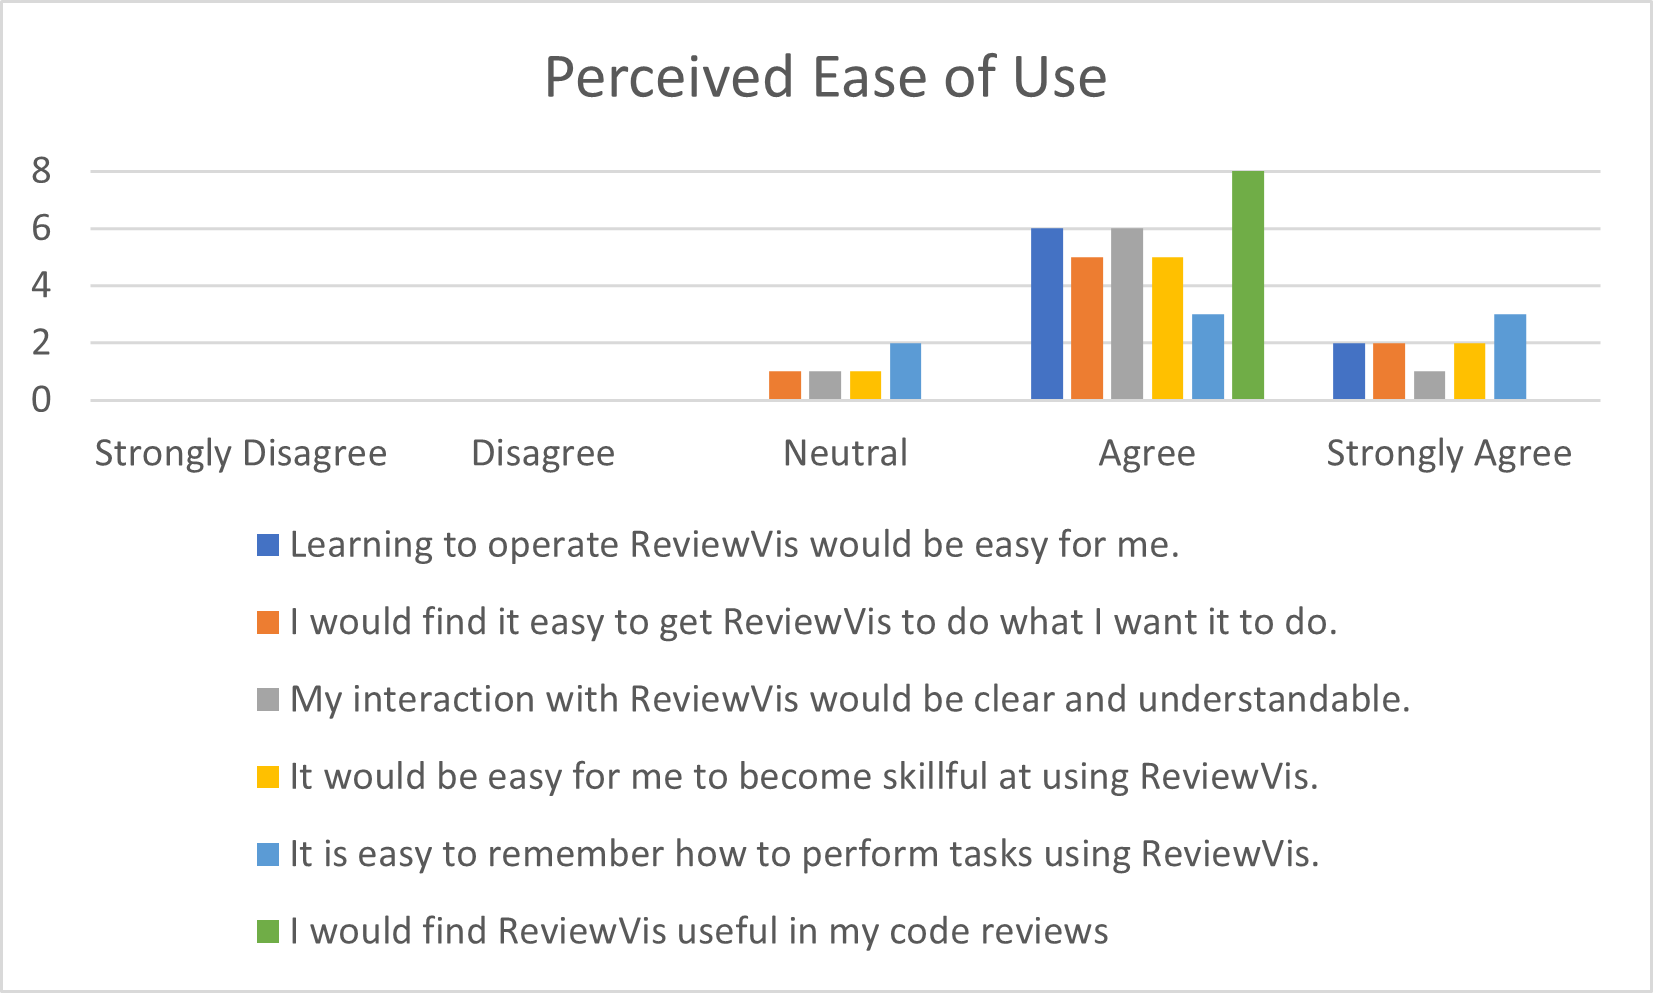
\includegraphics[width=1.0\textwidth]{Subfigures/perceived_ease_of_use.png}
    \caption{Ease of Use of ReviewVis as perceived by the participants.}
    \label{fig:PerceivedEaseOfUse}
\end{figure}

Figure \ref{fig:PerceivedEaseOfUse} summmarizes participants' perceived ease of use of ReviewVis. Overall participants thought that it would be easy to learn how to use ReviewVis, but they were not sure if they could remember how to do everything. Based on this we think that a short guide for users to reference will be enough to use the tool after a first introduction. This is consistent with answers from the interviews, where most developers answered that they need an initial explanation and maybe some time to fully understand and get used to it, but especially more experienced developers thinking they would learn it fast.


\paragraph{Settings} \label{Par:SettingsInterviews} 

Developers can choose between the change-based and a package-based coloring described in Section \ref{SubSubSec:FrontendSettings}. In evaluating them, all developers preferred the change-based coloring for code review. As such, this was made the default setting in later evaluations. When seeing the graph with change-based colors, many developers intuitively understood that green means the node was added and red that the node was deleted, but the meaning of orange (changed) sometimes needed to be explained. However, overall developers thought the coloring was clear. Package-based colors were seen as less useful because, as P2 put it: "\textit{Normally when doing code review I already have a grasp of the structure, so I would not use this feature.}" A possible application mentioned by P2 was tasks other than code review like reverse engineering, meaning that it is primarily useful when developers review code they are completely unfamiliar with.

A file can contain multiple warnings. A setting is provided to either show only one warning node per file with all warnings collected, or an additional warning node for each warning, which gets linked to the file warning node. Figure \ref{fig:warningExpandedComparison} shows a comparison. Feedback on this feature was mixed, with developers tending to prefer only one node to reduce clutter. P3 even wanted a way to hide all warnings, which is currently not possible.

\begin{figure}[h]
\centering
\begin{subfigure}{.5\textwidth}
  \centering
  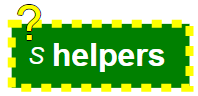
\includegraphics[width=0.3\linewidth]{Subfigures/warnings_final.PNG}
  \caption{One warning node per file.}
  \label{fig:combined-warnings}
\end{subfigure}%
\begin{subfigure}{.5\textwidth}
  \centering
  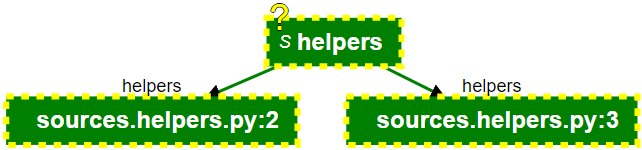
\includegraphics[width=0.9\linewidth]{Subfigures/warnings_final_expanded.PNG}
  \caption{One warning node per warning}
  \label{fig:expanded-warnings}
\end{subfigure}
\caption{Warnings indicating that the tool encountered a problem (e.g., could not resolve a call). There are two warnings for the file helpers, one for line 2 and one for line 3. In the settings the individual warning nodes can be toggled on or off.}
\label{fig:warningExpandedComparison}
\end{figure}

The tool provides a setting to show nodes not written in one of the supported programming languages (e.g., txt or xml files). Reviewers' feedback on this feature was mixed, with two saying that they would not use it, six saying that they think it’s useful, and four of them saying that it depends but that it’s good to have a choice. One developer mentioned that by being disconnected from the graph it doesn’t provide much information, but if usages in the code could be detected and displayed in the graph it would become interesting. 


\subsubsection{Reviewers' Perception of ReviewVis for Merge-requests Containing Python and Java} \label{SubSubSec:RQ1.2}

The tool offers two settings for how to handle graphs containing multiple languages. It can either open a new window for each language, each with its own graph. Or it can open only one window, with all language graphs distinguished by their border color of nodes and a toggle for the graph of each language. Figure \ref{fig:MultiLanguageExample} shows an example.
The feedback when comparing these two options was mixed. Generally, developers preferred having only one window, although three preferred multiple windows as well, with three participants also bringing up other approaches described at the end of this section. Overall, the interest in this feature was smaller, because while some thought it is useful, many developers rarely were in a situation where they reviewed code in multiple languages concurrently. An important application domain would probably be full-stack website development with different languages for the frontend and backend, which was not tested.

\begin{figure}[h]
    \centering
    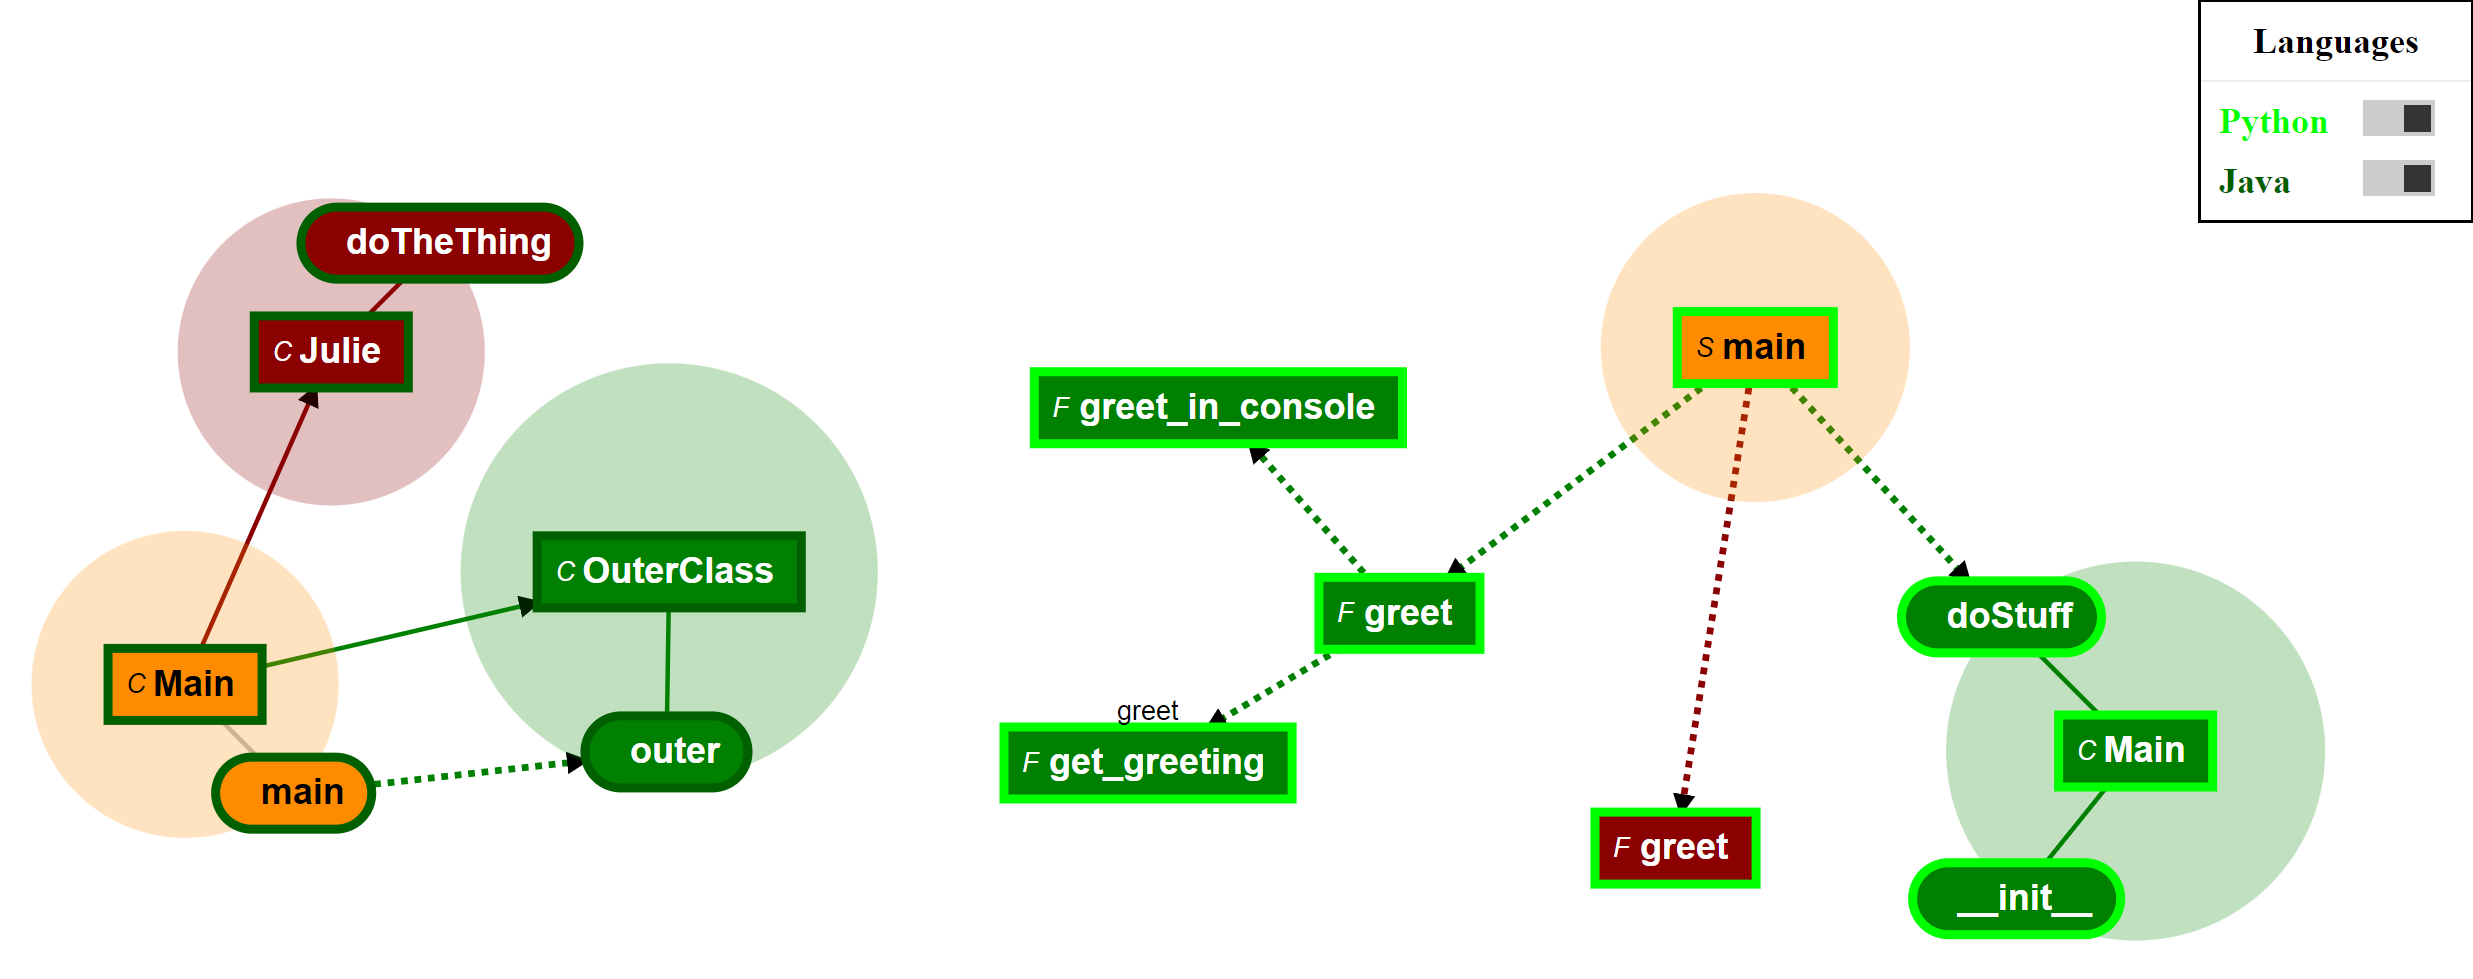
\includegraphics[width=1.0\textwidth]{Subfigures/multi_language_graph_example.png}
    \caption{Example for a graph containing nodes for both Python and Java.}
    \label{fig:MultiLanguageExample2}
\end{figure}

One important factor was the work setup: Developers with a smaller setup like a single laptop screen had less space for the graphs. Some preferred the combined approach, because this way they only had one window and could just toggle the languages on and off as needed. Others with a similar setup preferred multiple windows, because having multiple graphs in one small window was too large and would require a lot of zooming around. Developers with a multi-screen setup had more space for multiple windows, allowing them to arrange the windows as needed. Because the tool does not recognize connections between language graphs, this carries the same information as combining them. This meant that only a minority would display multiple graphs concurrently within the same window, with most preferring to instead toggle between them or splitting them up into separate windows. 

Another factor was the preference for less windows. Many participants expressed that they wanted less window management, which could be achieved by combining the graph. By allowing users to toggle the languages individually, some thought that they could do the code review in one window even if they wanted only one graph at the time. Also, combining everything into one window has the benefit that it is quicker to use due to not having to switch between windows, and it allows developers to more easily detect logical connections, even if the tool does not show them. Some also expressed that less windows but with more configuration options are better than multiple windows. 

Coloring the node border of each language in a different color was received well by developers. They thought it was intuitive, and one had the same idea when asked about possible solutions without being presented with the tool. Some said the link from colors to language was not clear, while others said it’s clear from context. To make it clearer for everyone, the colors were also added to the language toggles. In its current implementation the borders are only shown when more than one language is toggled on, but one developer expressed that they would like to have the colored borders always shown for multi-language graphs. 

Some ideas for other solutions were displaying both graphs in one window but enclosing each of them in a box to clearly separate them, and to separate them using tabs instead of fully separated windows. Using tabs would have the advantage of only being one window to manage, while at the same time making switching between languages quick and easy, and later participants who were asked about this thought it was a viable option.


\subsubsection{Future Work on ReviewVis to Better Support Developers During Code Review} \label{SubSubSec:RQ2}

In the interviews, we collected feedback regarding issues with the implementation of the tool as presented to the participants, as well as possible future improvements and features. In discussing them we also got some further insights into what developers value in a visualization tool for code review like the one we created. We first focus on what can be improved in the current state of the tool. Then we present features and changes requested by developers that can be implemented within ReviewVis. Lastly, we report where integration with other tools can improve support for developers during code review, and identify some areas outside of code review where code visualizations as implemented by ReviewVis could be useful. 

\paragraph{Directions for Improving the Current Implementation} \label{Par:CurrentImplementationIssues}

While many of the issues that came up during the interviews could be addressed, evaluated and further improved using the RITE approach, there remain some problems that we were not able to (fully) address due to time constraints and the complexity of the required changes. These should be addressed in further work on the tool. We focused on the tool and the visualizations itself, evaluating developers' opinion on it. But factors outside of it like toolchain integration are going to influence especially adoption rates, so this needs to be considered as well. 

The most common concern (mentioned by five interviewees) is the possible sub-optimal automatic positioning of nodes. The nodes are semi-randomly distributed within the window, starting with the main nodes (classes, etc.) and finishing with the method nodes. From there different forces move them into their final position. This approach does not take any of the relations into account. This is especially a problem for larger graphs. While there is not always a clear optimal positioning, the main metrics for a good graph extracted from the responses are tightly coupled nodes being positioned closely together and lines not crossing, the second one confirming the findings by Purchase et al. \cite{10.1007/BFb0021827}. Because this is one of the main issues brought up and as it impacts the core functionality of the tool, more advanced approaches to determine the optimal positioning would be one of the most important improvements that can be made. This includes determining what optimal positioning is, as it might require trade-offs between better node positioning and minimizing lines crossing.

As part of the RITE methodology, something that was done during the interviews to improve the visualization was to improve the positioning of methods around nodes: using the algorithm described in Section \ref{SubSubSec:RQ1.1}, they could be positioned closer to the most connected nodes within the class circle. For example, when a method calls another node that is below the parent classes node, it makes sense to position the method node below the parent closer to the called node. This improved the visualization for the medium sized examples, but for the large graph some developers still thought that it could be improved. The reason is that parent nodes (i.e., class, function and script nodes) can still be positioned far apart despite being connected, and crossing lines are not taken into account.

P6 mentioned the idea that the author could define an optimal layout for reviewers to use. However this can increase the authors' workload and might limit the applicability of the tool. Therefore it might be inferior to automatic solutions. Having good automatic positioning means that the tool would be more viable in scenarios where the user cannot interact with the graph (e.g., when only a picture of the graph is given), which will be discussed later in this chapter. 

When evaluated for a larger graph containing eleven class nodes, 3 developers also reported that the class nodes with their circles should be further apart by default, as some of them were quite large and overlapped with other circles. From the interviews we could not determine if this could also be solved by having smaller class circles. 

Another problem is that changes made to the graph cannot be easily undone, with some changes requiring a reload of the graph. For instance, developers would like to have a way to make a node name bold again to indicate that it was not yet reviewed, and showing hidden nodes. Especially the ability to hide nodes without indicating that any nodes were hidden was perceived as dangerous by two developers: reviewers might forget they decided to remove these nodes from the graph, and therefore not inspect them during the review. Having a list of hidden nodes or something similar from which they can be brought back could address this issue.


\paragraph{Requested ReviewVis Extensions} \label{Par:RequestedExtensions}

A primary direction for future work is including support for more programming languages: the currently supported languages cover only a minority of use cases, and most participant mentioned this as a limitation of the tool. This echoes the findings of Fröhlich et al. for Java \cite{cr_visualization_major}. Adding other (popular) languages would increase the range of projects in which this tool could be used. Guidance to select them could be taken from the TIOBE index\footnote{https://www.tiobe.com/tiobe-index/}, the RedMonk programming language rankings\footnote{https://redmonk.com/sogrady/2022/03/28/language-rankings-1-22/} and IEEE Spectrum\footnote{https://spectrum.ieee.org/top-programming-languages-2021}, which all rank C, C++, C\# and JavaScript (JS) in their Top 10 most popular programming languages. JS specifically, which is commonly used in combination with other languages for web development, would also enable researchers to better understand the appeal of the tool for multiple languages, at least when used for some web development projects.

One feature that was requested by P1 and which later participants expressed interest in when asked was a way to hide nested nodes (i.e., nodes contained within other nodes of the same type, such as functions defined within another function), for both functions and classes. Two different reasons were given for this: Three developers expressed that for graphs with a lot of nested nodes, it could become cumbersome to use and visually overcrowded. By only showing the top-level function or class, this could be prevented. The other factor was that the top-level node is the most important in the opinion of developers, with the nested nodes often only playing a supporting role for the parent or being used to structure code. As such, depending on the code, hiding them does not meaningfully reduce the information content of the graph. 

Another type of nodes that multiple developers expressed interest in hiding are deleted nodes. This could be done by using a toggle in the settings. The justification for this was that deleted nodes are of less interest, as they don’t represent any code that needs to be reviewed. By removing them from the graph its complexity is reduced, and the developers can focus on the important changes. Two out of three developers who supported this had relatively little experience with only 1-2 years of working experience. More experienced developers were split on the usefulness of such a feature: one reported that deletions are rare in established code bases, making such a feature less useful.

Another potentially useful feature that was reported by P8 was to have more fine-grained control for the type of unknown nodes for files not recognized by the tool in the graph. For example, while showing nodes written in languages not supported by the tool might still be of use, metadata files might not be. Adding a filetype-based white- or blacklist would enable a more fine-grained filtering of these nodes. This way, specific files like JS files could be included, while xml files could be excluded.

Developers were also asked about what they would think of adding more information to the graph using indicators on nodes, or showing more information when hovering over a node. The opinions on this depended on the type of information. For example, detecting errors in the code and displaying them in the tool was seen by five of the developers as potentially useful, while P4 said that it is “not really the point of the tool”. The same developer expressed that they would not be completely against more information, just that it really depends on what the information is. For example, something that was received well when discussed in the interviews are argument lists for function and method calls. All participants (except one) who expressed interest in this feature also said that the additional information should not use too much space or clutter the graph. For example, showing the information only when hovering over the corresponding node was seen as a potential solution. Adding toggles for such indicators would allow developers to select for themselves what information should be indicated in the graph, and to adjust to specific graphs as needed.

Overall, when talking about nodes and links in the graph, interviewees reported that they are important information and they generally would not hide them. Also, when they are hidden, the tool should clearly communicate this to the user. Many developers thought that hiding information can result in them forgetting about it, leading to problems. When the idea of automatically hiding some nodes for very large graphs came up, developers answered that it could be useful. However, it would need to be clearly indicated, and they must be able to display any hidden information (e.g. nested nodes) again. This might be achievable with existing features like hiding methods and settings to hide nested nodes, but would need to be evaluated in further studies. 

A potential feature that was brought up was a way to recognize renames and indicate them in the graph. The idea was that instead of having a deleted node with the old name and an added node with the new name, there would be a single changed node with a name like oldName->newName. When asked about this idea, especially developers with less experience (<2 years) were interested in such a feature, while more experienced developers (>5 years) were more alert towards potential issues. The most important factor for the more experienced developers was that this feature must be reliable. It would need to depend on some kind of heuristic to detect renames, which might be wrong. They also said that the way the tool works currently is very clear (meaning clear rules), while complicated processing might end up making the graph harder to understand. As one developer noted, it can also lead to a loss of information when it is not only a simple rename, but also contains added or deleted relations, which would not be distinguishable in the graph. Another developer who liked the idea brought up the possibility of a rename relation, but said that this could make the graph more complicated. 

Currently the change-based color scheme shows the additions, changes and deletions, while the package-based color scheme shows the package or file level structure of the graph. While all participants preferred the change-based color scheme, some thought that the package-based color scheme could also provide valuable information. However, currently users can only choose one of them and not use them simultaneously. An idea that P8 had is to have the nodes using one color scheme and adding borders with the other color scheme. This would combine the two, and could be a third option for developers to choose from. When combined with the approach for multiple languages in one window, which also uses border colors, this would have to be replaced by another approach like dotted or doubled borders, which could become overwhelming for reviewers. 

Another color scheme that was requested was a colorblind accessibility mode. For change-based coloring, red and green are used which are intuitively understandable, but can be hard for red-green colorblind people to differentiate. And for automatic coloring like with package-based coloring, the color distribution is random which can introduce issues as well. To address this problem, a colorblind mode should be added with alternative coloring that is easy to differentiate. 

When it came to the way code is currently visualized, two developers said that an alternative visualization scheme for certain types of code could be interesting, mainly tests. Tests have a different structure and function to normal code, and as such could benefit from specialized features. However, no concrete examples were given. 

One information that would be interesting to have in the graph is the change size. In its current implementation, large changes (spanning a large percentage of the total code) look the same as one-line changes in the graph. This way developers can see where the major changes were made and focus their attention on them. What information and how to communicate it exactly would need to be further researched, but some proposals are a percentage or LOC (lines of code) changed vs LOC total, or to communicate LOC added and removed separately. 

The size of the circle around main nodes is currently proportional to the name length (i.e., longer names correspond to larger circles). But as P6 mentioned, circle size carries a lot of information, as larger circles which take up more screen space indicate higher importance. To make better use of circle size, it could be tied to the LOC or number of methods of the class, which would be the most intuitive in the opinion of the developer who brought it up, but might not be very useful information. Other ideas to use it include change size, either with bigger circles corresponding to larger change sizes or two concentric circles indicating LOC added and removed. The circle size would need to be normalized, because the information communicated might differ by order of magnitudes (e.g., single-line code change vs hundreds of lines rewritten). Also, a later developer thought that using the circle size to communicate more information would not be a good idea, but admitted that they would have to see the actual implementation.


\paragraph{Integration With Other Tools and Use Cases Other Than Code Review} \label{Par:IntegrationOtherTools}

Focusing on code review, integrating information from other sources into the tool can be very useful in the opinion of five developers. One example is showing the result of static analysis tools like SonarCube\footnote{https://www.sonarqube.org/}, which statically checks code quality, within the graph. But it is important that they do not hinder developers in using the tool to obtain a light-weight overview of a code change, which is seen by developers as its core strength. For indicators (i.e., little symbols added to nodes, like the comment indicator), adding toggles to turn them off and on individually would be a good solution, allowing developers to be flexible in their tool choice and usage. An alternative would be hover text, which does not add visual information and as such reduces the risk of information overload. Finding ways to best integrate information into the existing tools and what information is most useful should be researched further.

Developers were also interested in how the tool could be integrated into their workflows. They expressed that using the tool should not hinder them in their work, meaning that it is easy to set up and can be used with little if any additional effort. Toolchain integration is, in their opinion, a major factor in the adoption of the tool in practice.

A popular request was expanding the tool for more use cases beyond strictly support for code review. This includes situations where the tool is used standalone (i.e., independently of GitLab, without being linked to the analyzed code) when only a high-level understanding of the code structure is needed.

One example is integrating the tool into Jira\footnote{https://www.atlassian.com/software/jira}, a task tracking platform P7 mentioned when talking about their workflow. Their company splits work into tasks and assigns them to developers, with other developers reviewing the changes made. They wanted to have a picture of the graph on completed tasks to show how the change was structurally implemented (e.g. a single large class, multiple small classes or functions). This way they could see a quick overview without having to leave Jira.

Other than that, developer P2 mentioned that it could be very interesting for reverse engineering, as it provides a high-level overview over the code structure. And P5 mentioned that it could be interesting to compare arbitrary branches in GitLab to see how ongoing development in them has led to divergent graphs, or to see what has been done so far. This is not directly related to code review, but shows that a tool like ReviewVis can effectively communicate information which could be useful in other aspects of software engineering. Applications of this tool beyond code review should be explored further in future studies. 

\newpage


\section{Limitations} \label{Sec:ThreatsValidity}

In the following sections we discuss both internal and external possible threats to validity. We also explain how we tried to mitigate known effects and discuss the possible impact of decisions when this was not possible.


\subsection{Internal Threats to Validity} \label{SubSecr:InternalThreatsValidity}

\subparagraph{Participant Selection}
The participants were selected partially from the professional networks of the authors. They were recruited by contacting them directly, explaining the study and asking them if they would be willing to participate. It is possible that participants were more likely to join because they felt pressured to do so. To mitigate this effect, it was made clear to participants that they could drop out of the study at any time, without providing any reason.

\subparagraph{Lack of Interaction}
The interviews were done remotely, with the tool running on the interviewers’ machine and the screen being shared with the participants. Because the focus of the tool was on the visualization, which were fully visible, this did not impact most of the interview. The interactions had to be explained and shown to the participants instead of them trying them out for themselves. Since the interactions only require one or at most two actions (clicking, clicking and moving mouse, scrolling) and therefore are relatively simple, they are easy to explain and understand. Furthermore, the effect of the interactions can be seen by the participants. However, we cannot exclude the remote nature of the evaluation might have introduced bias in the participants’ evaluation of the tool.

\subparagraph{Sample Merge Requests}
The merge requests used for the interviews were chosen by the author and the same ones were used for all interviews to make comparisons possible. They were selected to provide examples for different scenarios and to show all features of the tool. We believe that the insights from the evaluation can be translated to general code reviews, because the examples include scenarios covering a significant number of real-world scenarios. If participants understood the tool well enough to evaluate it, we believe they could also estimate the tools performance in other scenarios which they had experienced previously. That said, future studies should be conducted to evaluate the tool for a wider range of scenarios.

\subparagraph{Interviewer Effects}
The interviews were conducted by the author of this thesis, who is familiar with the tool and has worked on it. This could influence how the tool was presented and the questions asked. To try and mitigate this, the questions were open-ended without presuming any opinion of the participants. Some participants personally knew the author, which could have biased them towards giving overly positive feedback. We tried to encourage honest feedback by stressing that the tool is still in development and explicitly asking for what participants disliked.

\subparagraph{Evaluation Time}
The tool was introduced during the interviews, and participants had limited time to evaluate it. The evaluation happened also only during one period, the interview, instead of over a longer time period. Some participants further evaluated the tool on their own, and some additional feedback could be given in the questionnaire, but this was limited.


\subsection{External Threats to Validity} \label{SubSec:ExternalThreatsValidity}

\subparagraph{Experimenter Effect}
The author of this thesis was also the primary interviewer, which might have influenced the interviews. To mitigate it, somebody else with research and interviewing experience sat in on some of the interviews to ensure that any possible influences were limited.

\subparagraph{Sampling Bias}
Participants were recruited from the professional network of the authors. It is possible that this could have introduced some bias concerning the selected participants. By selecting participants from multiple companies and contexts, as well as including some participants from other channels, we tried to mitigate any possible biases. However, we cannot exclude that the limited sample of participants selected might have influenced our findings. Further studies should be conducted to strengthen the generalizability of our findings.

\newpage


\section{Discussion} \label{Sec:Discussion}
In this chapter we discuss the insights and results obtained from the interviews. We present recommendations for future work based on our findings.

\subparagraph{Support for More Programming Languages}
Developers reported that support for more programming languages should be one of the primary areas of future work. This echoes the prior findings for Java \citep{cr_visualization_major, publication-20661}. Adding other (popular) languages would increase the range of projects in which this tool could be used. Guidance to select them could be taken from the TIOBE index\footnote{https://www.tiobe.com/tiobe-index/}, the RedMonk Programming Language Rankings\footnote{https://redmonk.com/sogrady/2022/03/28/language-rankings-1-22/} and IEEE Spectrum Top Programming Languages\footnote{https://spectrum.ieee.org/top-programming-languages-2021}, which all rank C, C++, C\# and JavaScript (JS) in their Top 10 most popular programming languages as of the time of writing.
JS specifically, which is commonly used in combination with other languages for web development, would also enable researchers to better understand the appeal of the tool for multiple languages, at least when used for some web development projects.

Thanks to the work done for this thesis, the CDV frontend can support most modern programming languages. For the CDP backend, a separate parser needs to be implemented for each language. To integrate them all, the Language Server Protocol (LSP)\footnote{https://www.langserver.org/} could be used, which supports almost any language and instances of which can run in parallel.

\subparagraph{Technical Limitations}
Another area where more work can be done is to extend the support to more programs: Regarding version control systems, ReviewVis currently only supports GitLab. Extending it to other version control systems would allow it to be used more broadly. Because it is mostly self contained, adding support for more platforms requires only punctual adjustments. Future work could implement an API for the features and interactions that need to interact with the platform (i.e., graph-to-code, loading comments), with platform-specific adapters.
For browser support, ReviewVis supports Google Chrome, which is at the time of writing the most widely used webbrowser according to Kinsta\footnote{https://www.kinsta.com/browser-market-share/}. Nonetheless, ReviewVis could be extended to other popular browsers as well. As ReviewVis relies on HTML and JavaScript for its visualizations, which are browser agnostic, the tool itself would not need to be adjusted.

\subparagraph{Large changesets}
Participants consistently found the tool useful for changesets that were medium sized (around 5-15 nodes). For smaller changes the tool does not offer enough information, as developers expected to understand the changeset without it. Developers disagreed most about the usefulness for large changes: A complex graph is harder to understand. However, it corresponds to a larger and more complex code change, where tool support could be even more useful. This matches the findings by Fregnan et al., who found that ReviewVis was seen as most useful for large merge requests (8+ files), with a minority thinking it might not be useful \cite{cr_visualization_major}. 
An important factor that future work should focus on is improving automatic positioning of the nodes in the graph: tightly coupled nodes should be positioned close together, while minimizing crossing lines to improve understandability \cite{10.1007/BFb0021827}. And more general, research should explore in more detail what makes ReviewVis useful for large changes. We believe that graph complexity (i.e., number of nodes and interconnections) is a major factor in this, and a way to measure it and investigate see how it impacts usefulness would be helpful. This would improve our understanding of the tool and help guide the development of new features.

\subparagraph{Information Content}
Developers thought that the level of detail (i.e., how much information is presented) in the graph is at a good balance, providing enough information to be useful but not overloading it. Adding information was seen as potentially useful if it could be done without reducing visual clarity, for example by using hover text or opening a submenu when right-clicking a node. The focus there should be on information within the domain of the tool like function parameters, as opposed to information requiring complex heuristics like code errors. One option could be adding indicators (i.e., little symbols on specific nodes, like the comment indicator). This would be scaleable to other information, but might reduce visual clarity. Another option could using existing visualizations more effectively: One developer mentioned that the size of a node (especially class nodes with a circle around them) carries a lot of information (i.e., larger nodes are more important). Using this to communicate more information, for example as an indicator of change size within this node, would be interesting for future research.
Removing information could also be useful especially for complex graphs. Examples from the interviews would be options to hide nested nodes (functions and classes), or deleted nodes. But hiding information can be dangerous, so there needs to be a way to make the developer aware of hidden information and letting them display it. Overall, keeping the graph simple was seen as more important than adding more information. Future work could explore what additional information developers want, and how to display it in the visualization.

\subparagraph{Importance of Adaptability}
The perceptions of the tool were influenced by the experience and tools the participants used. For example, some projects are more fluid than others (resulting in more deletions), and tools and features like the option to hide deleted nodes would be primarily useful for these code bases. Similarly, deciding what information to show and how depends on the structure and type of the code (many small classes vs. larger classes, tests, etc.). The same is true for the work setup, with less screen space leading to developers preferring denser presentations. Prior experience with other tools also made developers think about how information from them could be integrated with ReviewVis. As these needs diverge and sometimes have oppositional preferences, a single implementation cannot be optimal for all users. This means that the tool should allow developers to adapt it to their needs and be flexible in how and for what it can be used.
Future studies should therefore investigate which features are the most important for developers. These should then be exposed to the user in the form of settings. As the feedback to the current implementation of settings (i.e., toggles in the browser) was positive, this approach could be used for additional settings. Less important settings can be grouped into submenus. Another possibility could also be a settings file. This could enable users to share settings they found to work well for their use case. The default settings, used when the tool is not set up yet, should be well-chosen based on prior feeedback on what is most useful and understandable.

\subparagraph{Requested Features}
When it came to adding advanced features to the tool that rely on heuristics (e.g. to find renames), many developers were skeptical that they would be unreliable or that it would be hard to understand how they work. As such they would be distracting or not trustworthy. Generally, they advised to prioritize the core strengths of the tool (static analysis to create an abstraction of the code change) over advanced features. Developers were more interested in the toolchain integration than in adding features to the tool itself. One aspect of this is to make the tool easy to use in their workflow, without (much) additional work, which confirms prior findings \citep{6606613, 10.1145/3188720}. By making it the default developers would be more likely to use it. Some participants also expressed interest in integrating ReviewVis in other tools and vice versa. For example, having a picture of the graph in Jira\footnote{https://www.atlassian.com/software/jira} (a task tracking website) to see implementation structure, or having it in their IDE. The other way around would be to indicate or show information from other tools like static analysis tools in the graph. However, this was controversial, with many thinking that this could add too much information.
   
\subparagraph{ReviewVis Beyond Code Review}
Multiple developers expressed interest in ReviewVis for use cases other than code review, and in the questionnaire participants found ReviewVis more useful for general applications than just using it for code review. One possible area where it could be useful would be for reverse engineering, where an overview of the structure of the code could be very useful. Another area was to use just pictures of the graph in other tools to give an overview without having to leave the other tool (preferably with improved automatic node positioning). We think this indicates that a graph-based visualization like ReviewVis has benefits like improved understanding of code that apply not only to code review, but other tasks as well. As such, this could be of interest for future research.

\newpage

 
 \section{Conclusion} \label{Sec:Conclusion}
 
 We extended and improved a tool for code review support called ReviewVis that uses a graph visualization to display dependencies and calls within the code. We added support for a second programming language, Python, and added support for functional programming paradigms. We also added support for doing code review in multiple languages concurrently. We then conducted a series of remote interviews to evaluate it, and iteratively improved it following a RITE-inspired methodology. In the interviews we focused on determining how reviewers perceive the tool when used for Python, what their opinion on the tool for code review in multiple languages was, and how the tool could be further improved. Furthermore, we evaluated the perception of the tool using the TAM model. Participants responded positively to the tool, preferring it over using just GitLab and predicting that they would use it. They found it easy to learn and especially useful for gaining an overview of code changes. Reviewers preferred a simple visualization in which they can selectively display more information, with the tool focusing on its core strengths of showing an abstraction of the code change without complex analysis. They advised to focus more on seamless integration into existing toolchains, and noted that such a visualization could also be useful in other areas where large changesets need to be understood. 

Future work on the tool should focus on extending tool support to more languages, as this is its primary limitation, and to improve node positioning to improve the visualization. After that, it should be explored in more details what the limitations of the tool for different code bases and change sizes are and how they can be addressed. Integrations into toolchains and other tools, not only for code review but for other areas where visualizations could help code understanding, was seen as an important factor for adoption and usefulness.


\newpage
% If your text finishes on the even page, comment the following block before \appendix.
\thispagestyle{empty} % Comment this if your text finished on the odd page.
\cleardoublepage

% Before adding  Bibliography we are making sure 
% that it is going to be added to the table of contents.
\phantomsection % to enable hyperlinking in the ToC since "hyperref" package is used
\addcontentsline{toc}{section}{References}
\bibliography{thesis-bib}
% If your text finishes on the even page, comment the following block before \appendix.
\newpage
\thispagestyle{empty} % Comment this if your text finished on the odd page.
\cleardoublepage


% This command creates an appendix
\appendix

\section{Consent Form} \label{App:ConsentForm}

\includepdf[pages={-}]{Subfigures/Appendices/Participant_Consent_Form.pdf}

\section{Interview Structure} \label{App:InterviewStructure}
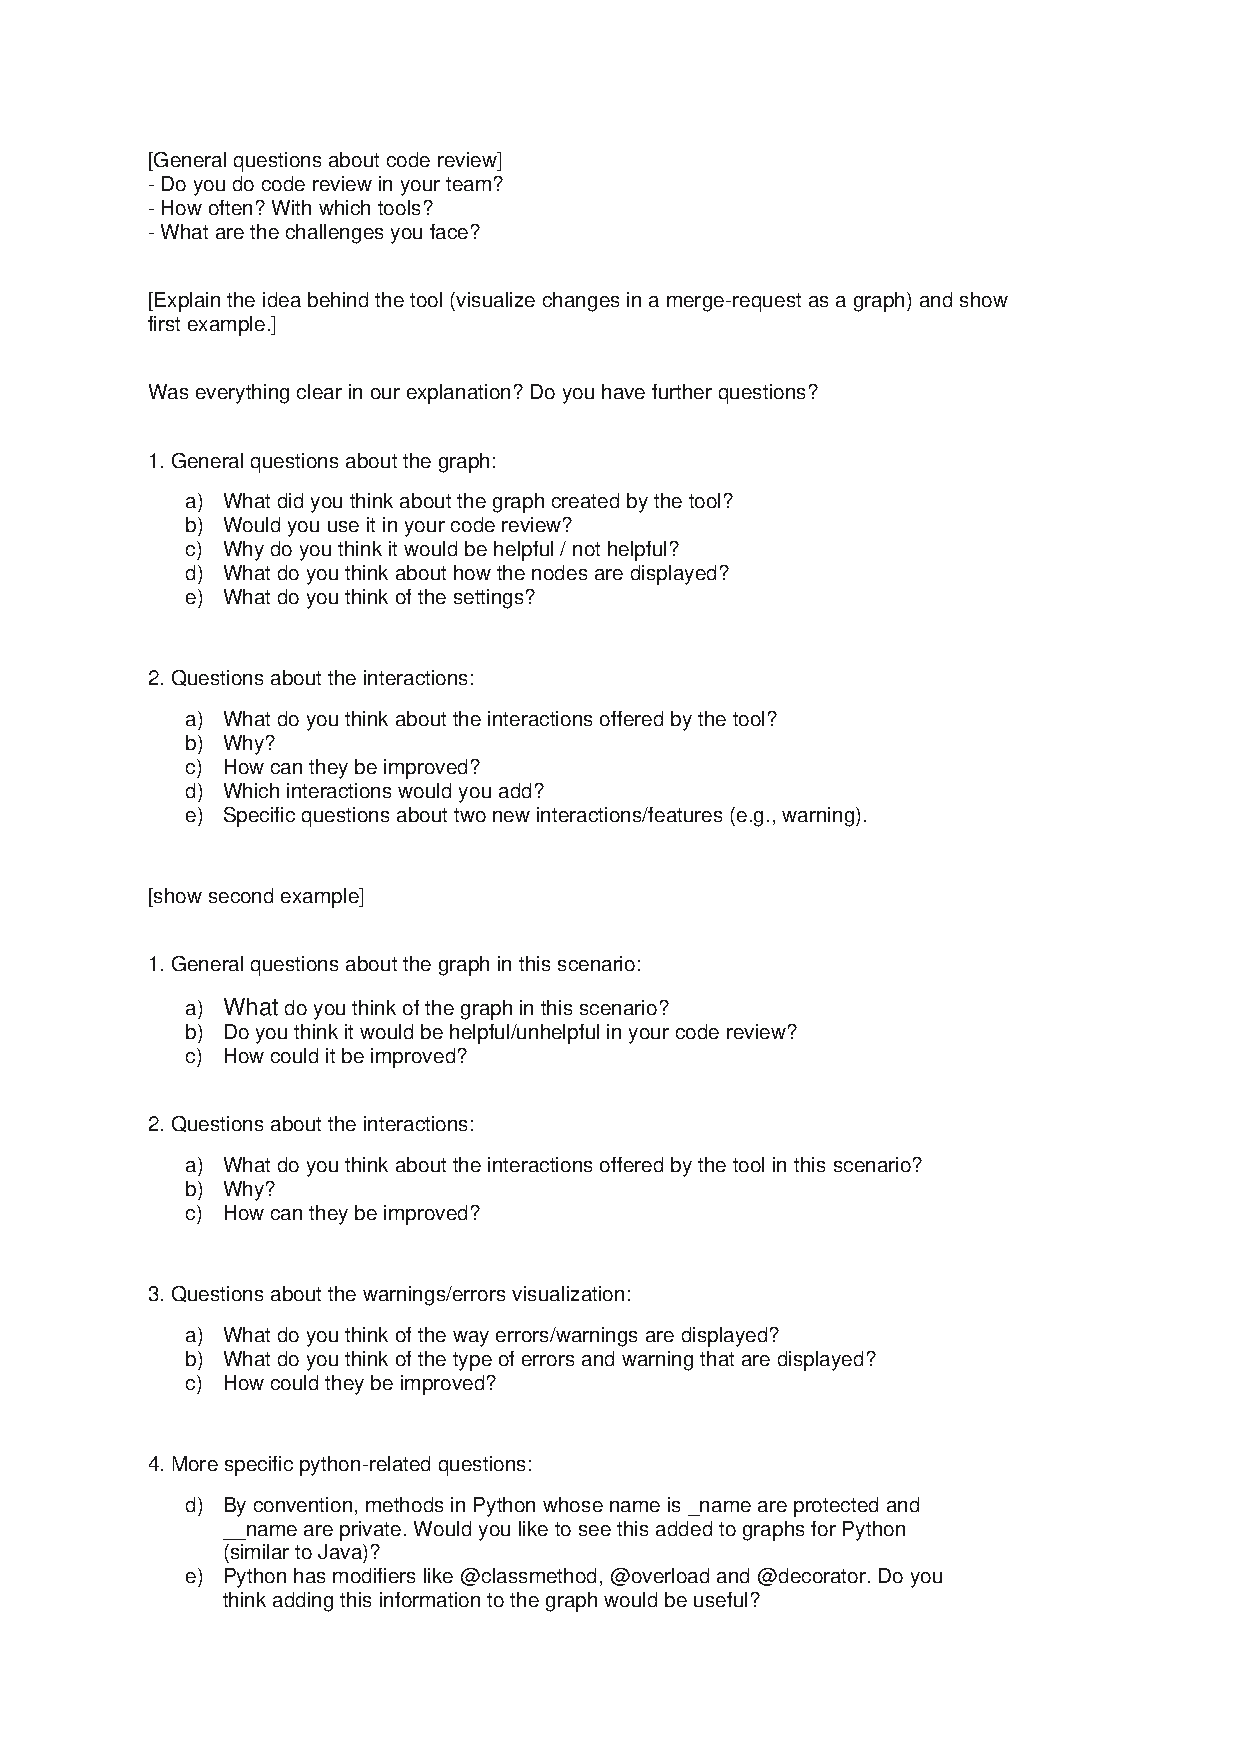
\includepdf[pages={-}]{Subfigures/Appendices/Interview_Structure.pdf}


\section{Interview Example Graphs} \label{App:InterviewExampleGraphs}
\captionsetup[figure]{list=no}
\begin{figure}[h]
    \centering
    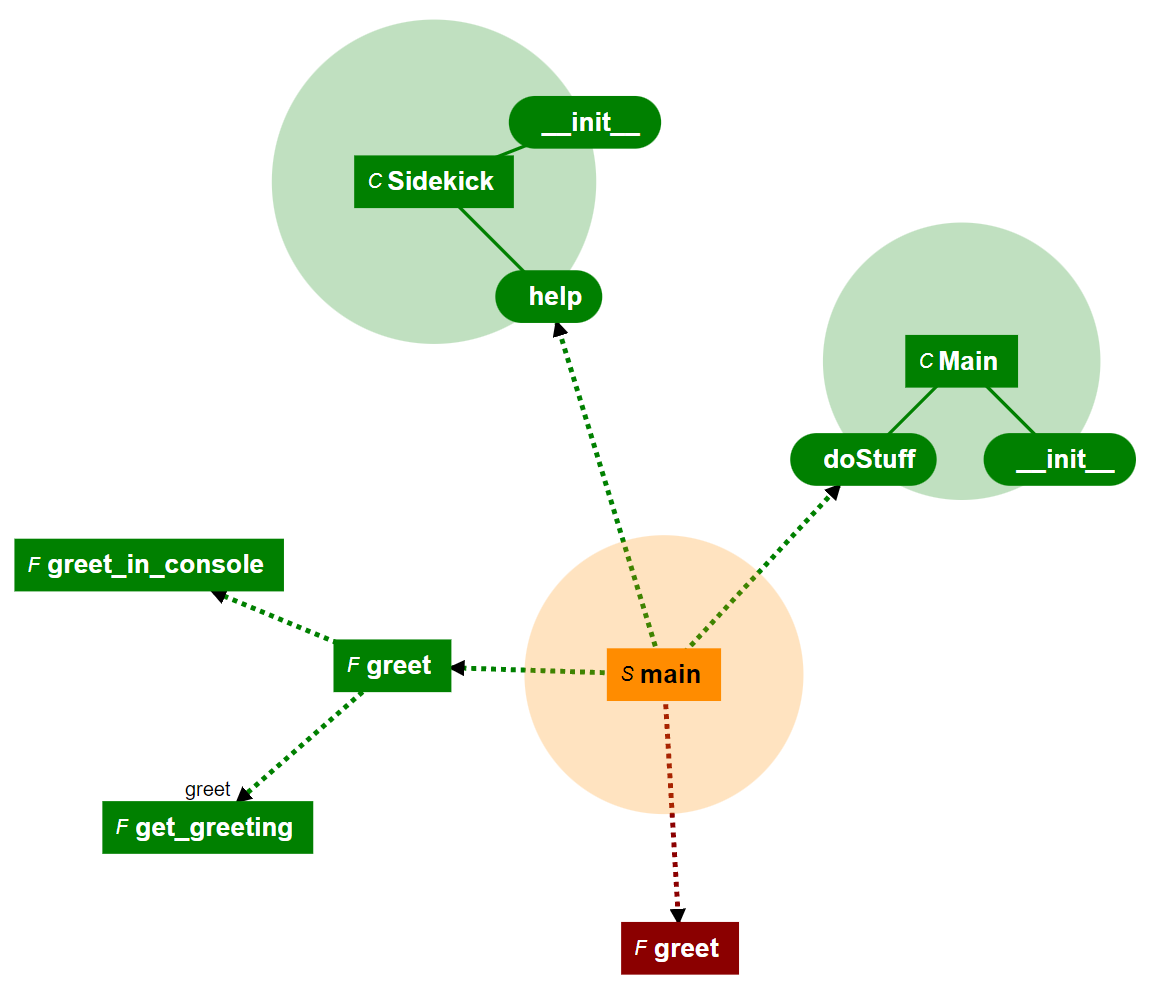
\includegraphics[width=1.0\textwidth]{Subfigures/Appendices/Interview_Examples/example_small.PNG}
    \caption{Smaller introductory example.}
\end{figure}

\begin{figure}[h!]
    \centering
    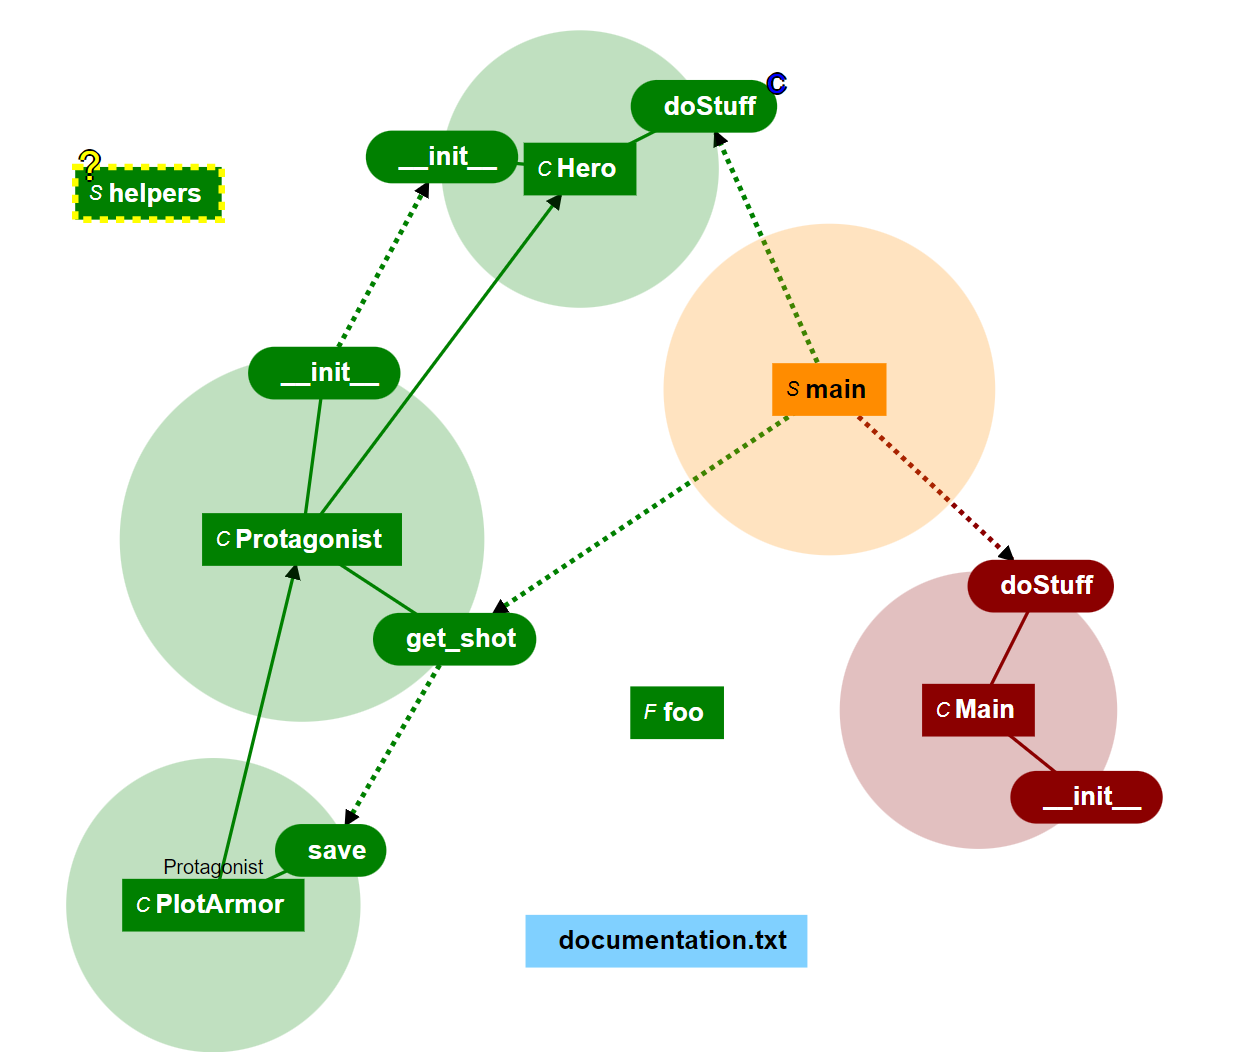
\includegraphics[width=1.0\textwidth]{Subfigures/Appendices/Interview_Examples/example_big.PNG}
    \caption{Example for a graph with more elements (warnings, unknown files, comments, ...).}
\end{figure}

\newpage

\begin{figure}[h!]
    \centering
    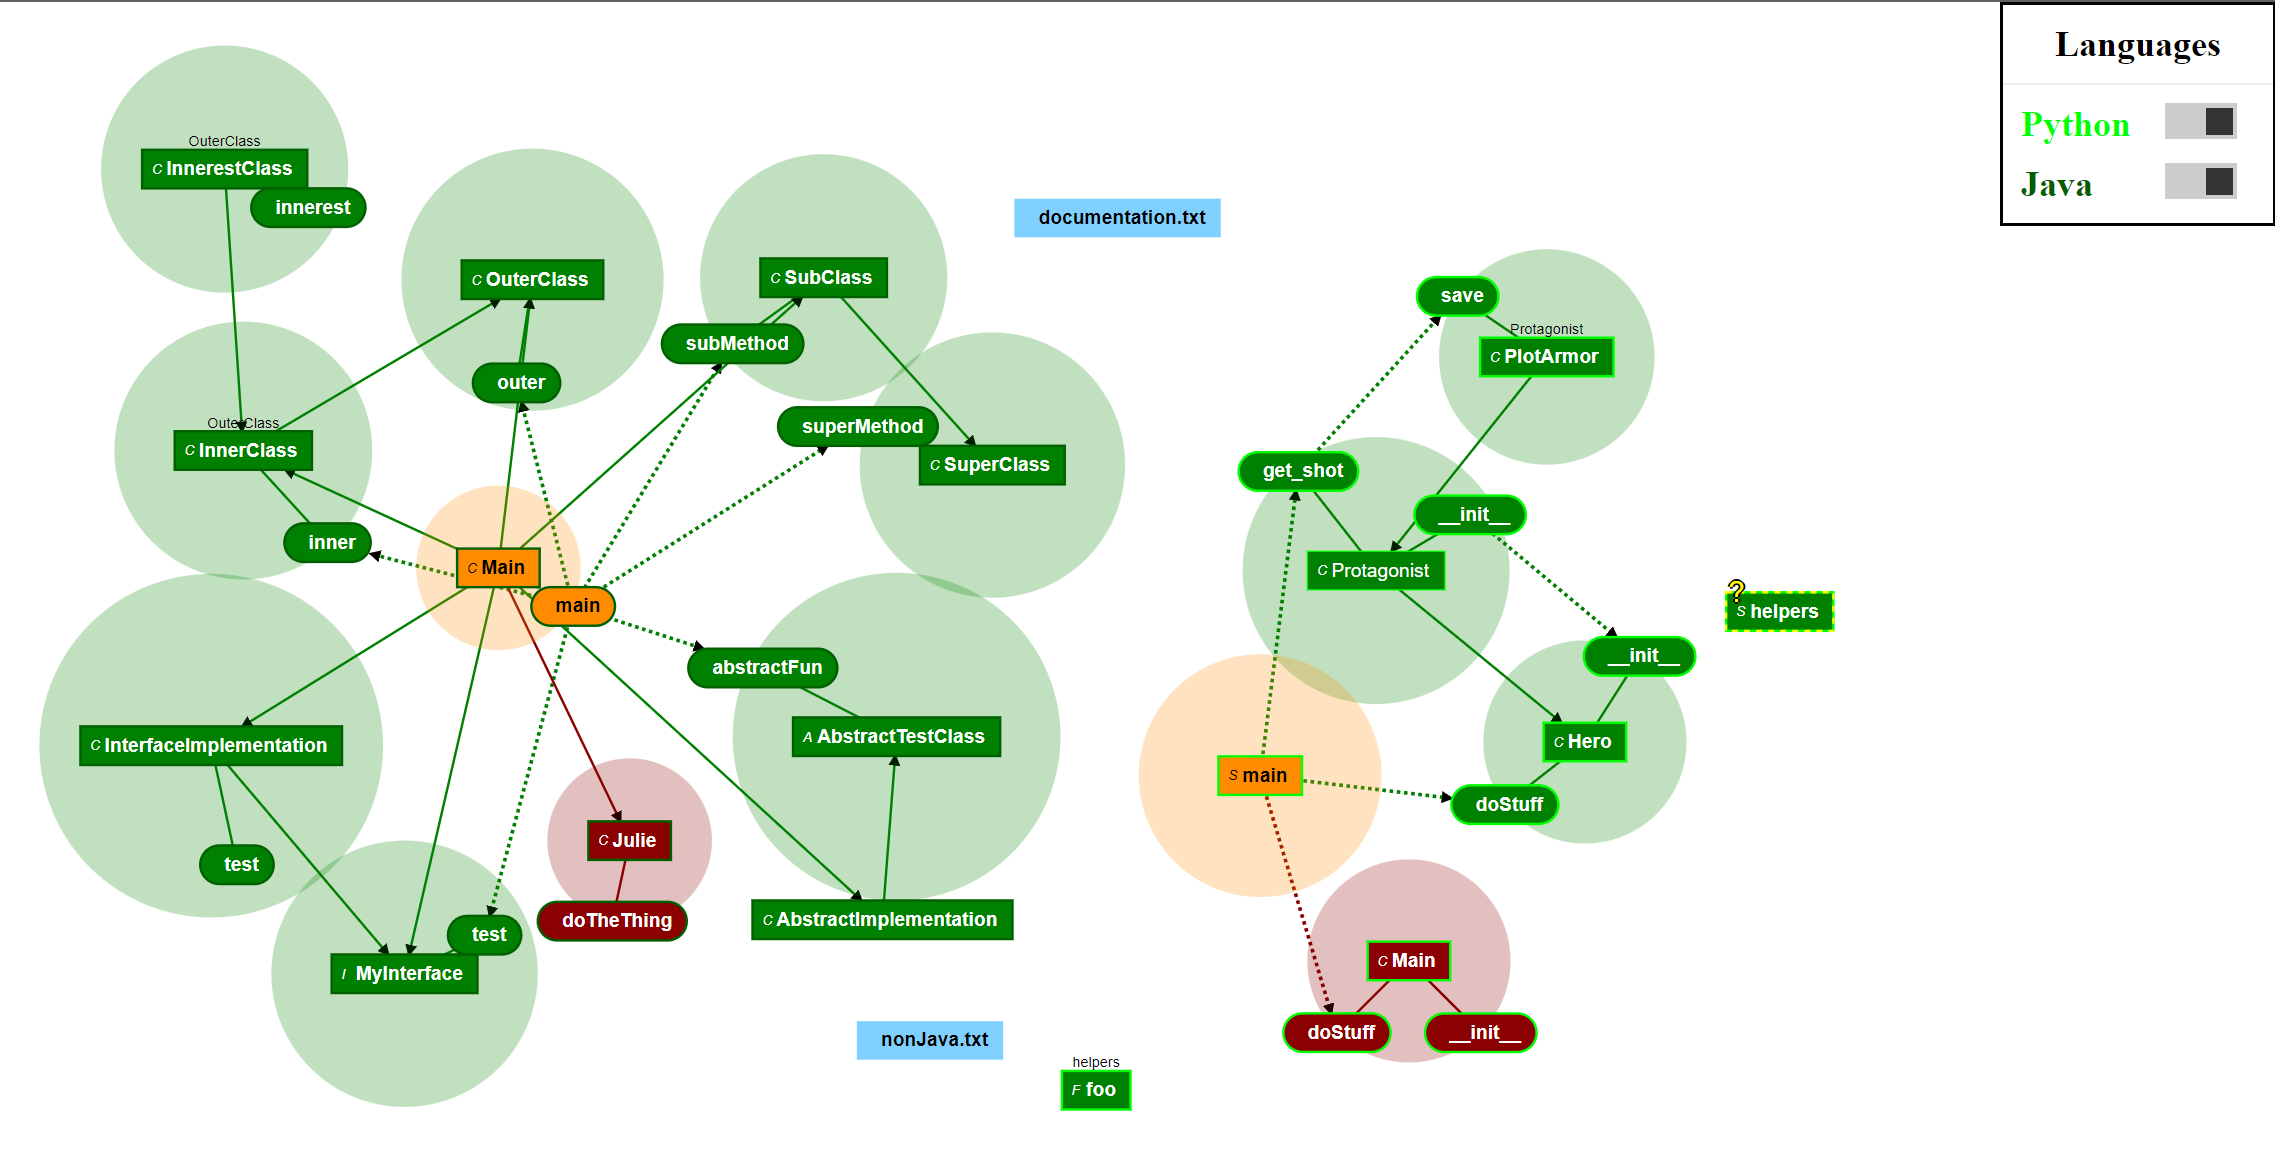
\includegraphics[width=1.0\textwidth]{Subfigures/Appendices/Interview_Examples/example_combined.PNG}
    \caption{Example combining Python and Java.}
\end{figure}


\section{Questionnaire} \label{App:Questionnaire}

\begin{figure}[h]
    \centering
    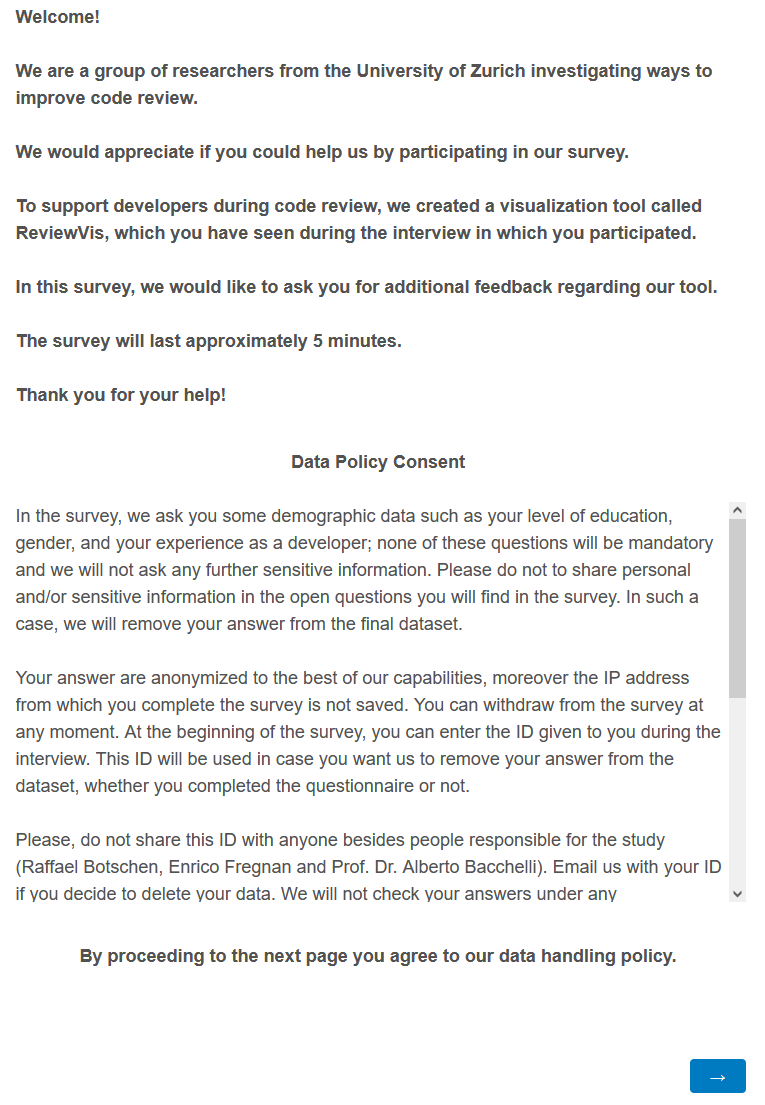
\includegraphics[width=0.8\textwidth]{Subfigures/Appendices/Questionnaire/questionnaire_1.PNG}
\end{figure}

\begin{figure}[h]
    \centering
    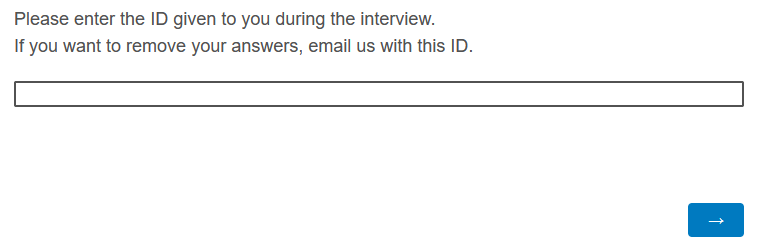
\includegraphics[width=1.0\textwidth]{Subfigures/Appendices/Questionnaire/questionnaire_2.PNG}
\end{figure}

\begin{figure}[h]
    \centering
    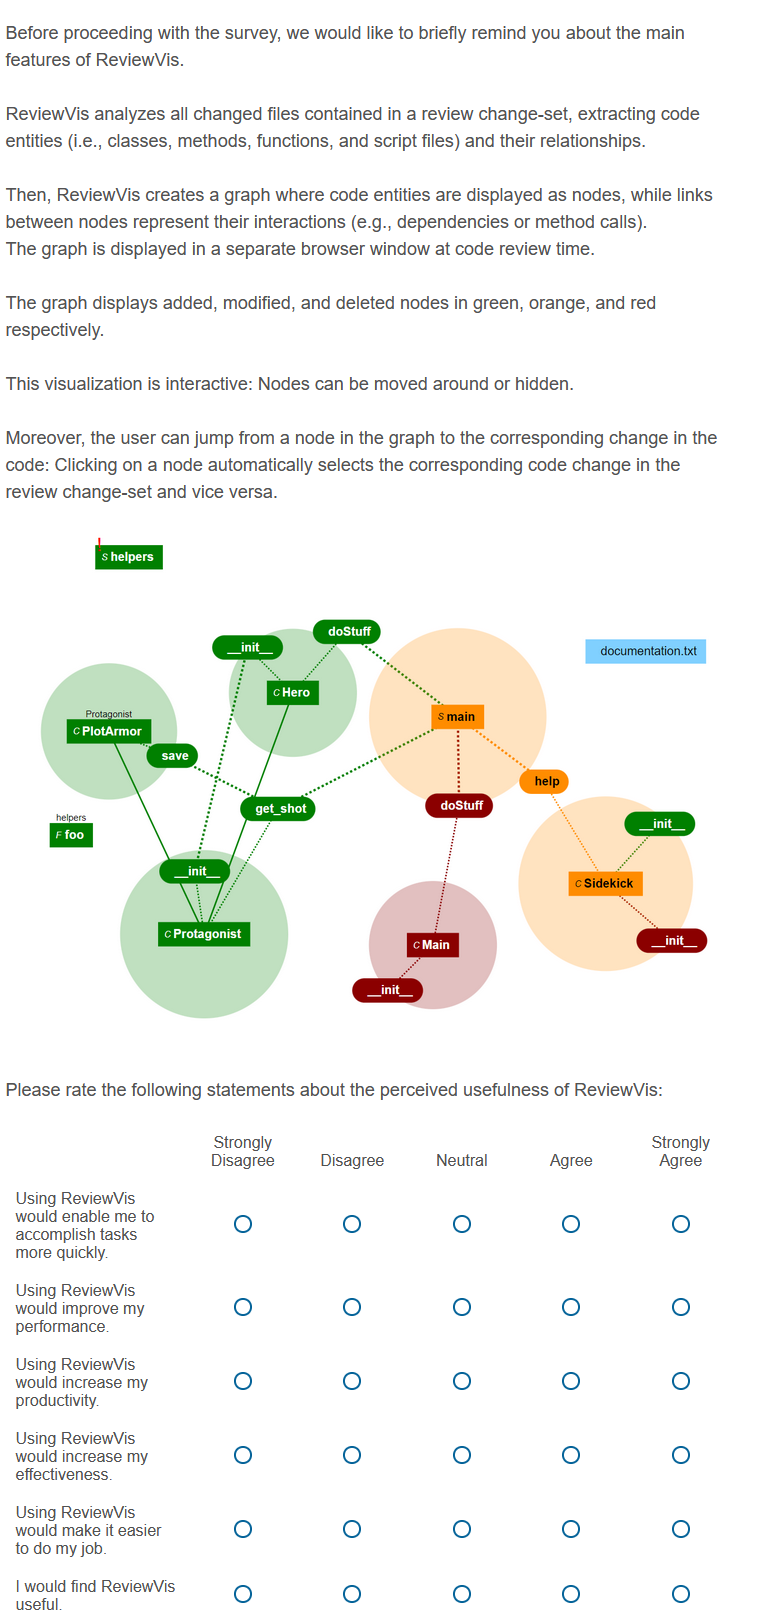
\includegraphics[width=0.8\textwidth]{Subfigures/Appendices/Questionnaire/questionnaire_3.PNG}
\end{figure}

\begin{figure}[h]
    \centering
    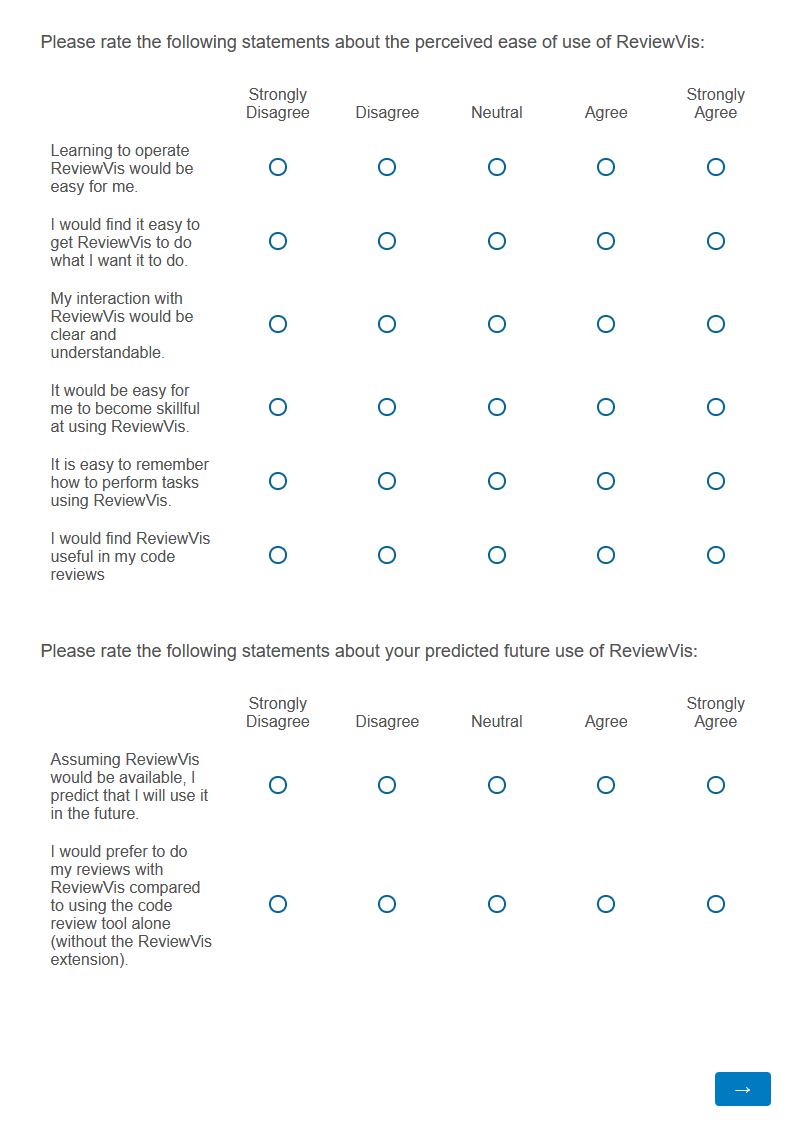
\includegraphics[width=1.0\textwidth]{Subfigures/Appendices/Questionnaire/questionnaire_4.PNG}
\end{figure}

\begin{figure}[h]
    \centering
    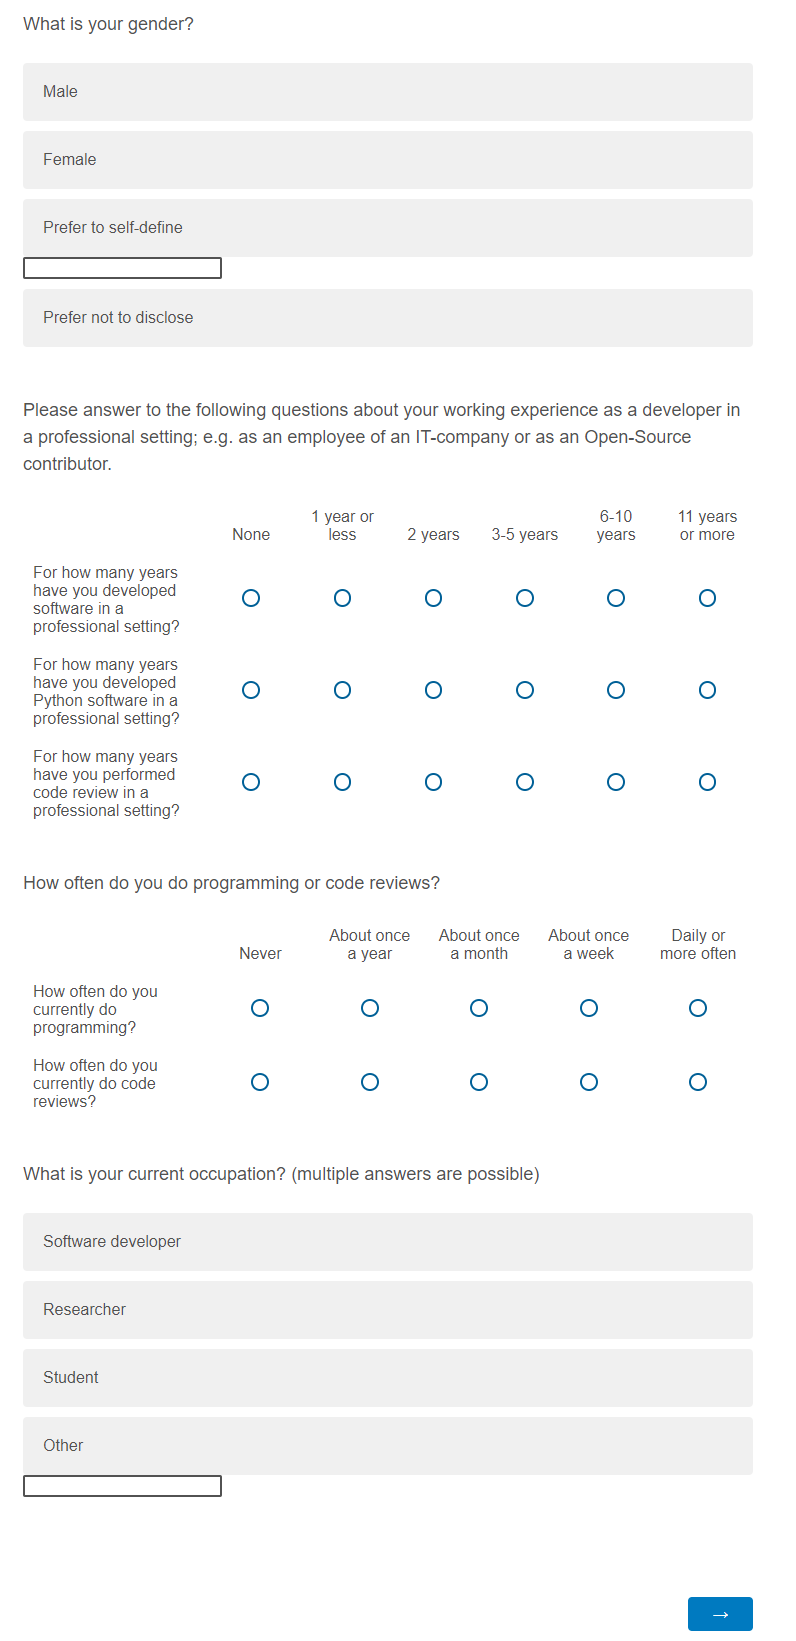
\includegraphics[width=0.8\textwidth]{Subfigures/Appendices/Questionnaire/questionnaire_5.PNG}
\end{figure}

\begin{figure}[h]
    \centering
    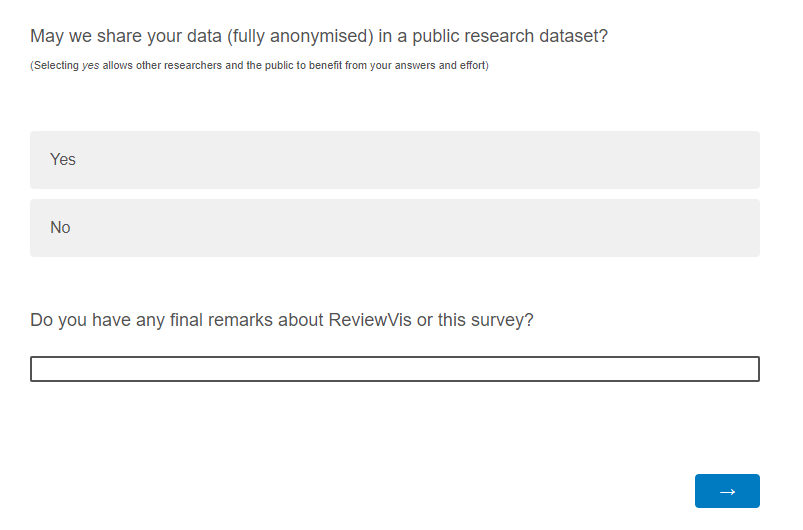
\includegraphics[width=1.0\textwidth]{Subfigures/Appendices/Questionnaire/questionnaire_6.PNG}
\end{figure}

\end{document}